% Created 2019-01-23 Wed 08:41
% Intended LaTeX compiler: pdflatex
\documentclass[11pt]{article}
\usepackage[utf8]{inputenc}
\usepackage[T1]{fontenc}
\usepackage{graphicx}
\usepackage{grffile}
\usepackage{longtable}
\usepackage{wrapfig}
\usepackage{rotating}
\usepackage[normalem]{ulem}
\usepackage{amsmath}
\usepackage{textcomp}
\usepackage{amssymb}
\usepackage{capt-of}
\usepackage{hyperref}
\author{Martin Nørskov Jensen}
\date{\today}
\title{}
\hypersetup{
 pdfauthor={Martin Nørskov Jensen},
 pdftitle={},
 pdfkeywords={},
 pdfsubject={},
 pdfcreator={Emacs 26.1 (Org mode 9.1.5)}, 
 pdflang={English}}
\begin{document}

\tableofcontents

\section{Introduction (1)}
\label{sec:org7b3051b}
\begin{figure}[htbp]
\centering
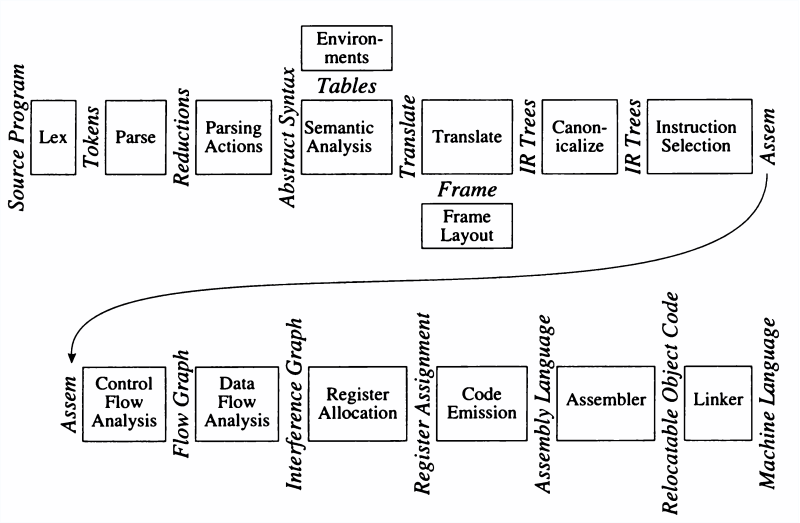
\includegraphics[width=.9\linewidth]{Introduction (1)/screenshot_2018-09-04_08-35-20.png}
\caption{\label{fig:org56bcff2}
Phases of a compiler and interfaces between them}
\end{figure}

\section{Lexical Analysis (2)}
\label{sec:org384e16c}
\subsection{General}
\label{sec:orgdd2482c}
\begin{itemize}
\item The analysis of a program is usually broken into
\begin{itemize}
\item \textbf{Lexical analysis:} breaking the input into individual words or "tokens"
\item \textbf{Syntax analysis:} parsing the phrase structure of the program
\item \textbf{Semantic analysis:} calculating the programs meaning
\end{itemize}

\item The lexical analyzer takes a stream of characters and produces a stream of names, keywords and punctuation marks
\begin{itemize}
\item It discards white space and comments between tokens
\end{itemize}
\end{itemize}

\subsection{Lexical Tokens}
\label{sec:org5054e00}
\begin{itemize}
\item A \textbf{lexical token} is a sequence of character that can be treated as a unit in the grammar of a programming language.
\begin{itemize}
\item A programming language classifies lexical tokens into a finite set of token types
\end{itemize}
\end{itemize}

\begin{figure}[htbp]
\centering
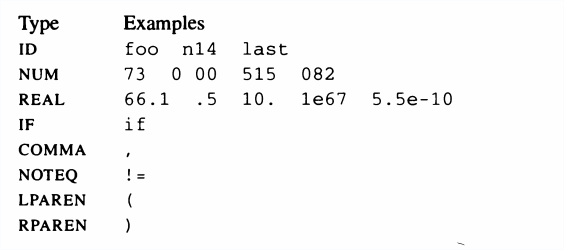
\includegraphics[width=.9\linewidth]{Lexical Analysis (2)/screenshot_2018-09-04_08-50-30.png}
\caption{\label{fig:org496fbfd}
Examples of token types}
\end{figure}

\begin{itemize}
\item Punctuation tokens such as \texttt{IF}, \texttt{VOID}, \texttt{RETURN} constructed from alphabetic characters are called reserved words and can in most languages not be used as IDs
\end{itemize}

\begin{figure}[htbp]
\centering
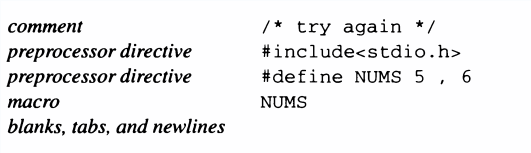
\includegraphics[width=.9\linewidth]{Lexical Analysis (2)/screenshot_2018-09-04_08-50-46.png}
\caption{\label{fig:org73e86b2}
Examples of nontokens}
\end{figure}

\subsection{Regular Expressions}
\label{sec:org5967269}
\begin{itemize}
\item A lexer is defined in the book using regular expressions and a FA.

\item There are two important disambiguation rules used by Lex, ML-Lex and other similar lexical analyzer generators
\begin{itemize}
\item \textbf{Longest match:} The longest initial substring of the input that can match any regular expression is takes as the next token
\item \textbf{Rule priority:} For a \emph{particular} longest initial substring the first regular expression that can match determines its token type
\begin{itemize}
\item This means that the order of writing down the regular expression rules has significance
\end{itemize}
\end{itemize}
\end{itemize}

\subsection{FA}
\label{sec:org27073a2}
\begin{itemize}
\item To recognize the longest match just means remembering the last time the automaton was in a final state with two variables, \texttt{Last-Final} (the state number of the most recent final state encountered) and \texttt{Input-Position-at-Last-Final}
\begin{itemize}
\item Every time it enters a final state it updates the variables
\item When a \emph{dead} state (a nonfinal state with no output transitions) is reached the variables tell that the token was matched and where it ended
\end{itemize}
\end{itemize}

\subsection{ML-Lex: A Lexical Analyser Generator}
\label{sec:org39904be}
\begin{itemize}
\item ML-Lex is a lexical analyser generator that produces a ML program from a lexical specification

\item For each token type in the programming language to be lexical analysed the specification contains a regular expression and an action
\begin{itemize}
\item The action communicates the token type to the next phase of the compiler
\item The output of ML-Lex is a program in ML that interprets a DFA
\end{itemize}
\end{itemize}

\begin{figure}[htbp]
\centering
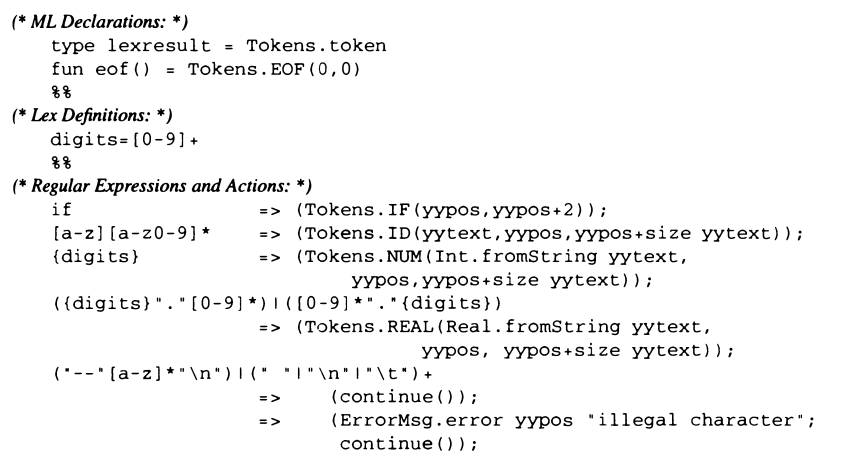
\includegraphics[width=.9\linewidth]{Lexical Analysis (2)/screenshot_2018-09-04_09-59-26.png}
\caption{\label{fig:org49af8c4}
An example of an ML-Lex specification}
\end{figure}

\begin{itemize}
\item The first part of the specification contains functions and types written in ML
\begin{itemize}
\item These must include the type \texttt{lexresult} which is the result type of each call to the lexing function
\item It must also include the function \texttt{eof}, which the lexing engine will call at end of file
\end{itemize}

\item The second part of the specification contains regular-expression abbreviations and state declarations
\begin{itemize}
\item e.g. \texttt{digits=[0-9]+ allows the name \textasciitilde{}\{digits\}} to stand for a nonempty sequence of digits within regular expressions allows
\end{itemize}

\item The third part of the specification contains regular-expression abbreviations and state declarations
\begin{itemize}
\item The actions are fragments of ordinary ML code
\item Each action return a value of type \texttt{lexresult}
\item In the action fragments, several special variables are available
\begin{itemize}
\item The string matched by the regular expression is \texttt{yytext}
\item The file position of the beginning of the matched string is \texttt{yypos}
\item The function \texttt{continue()} calls the lexical analyser recursively
\end{itemize}
\end{itemize}

\item It is possible to declare a set of \emph{start states}
\begin{itemize}
\item Each regular expression can be prefixed by the set of start states in which it is valid
\item The action statements can explicitly change the start states
\end{itemize}
\end{itemize}

\begin{figure}[htbp]
\centering
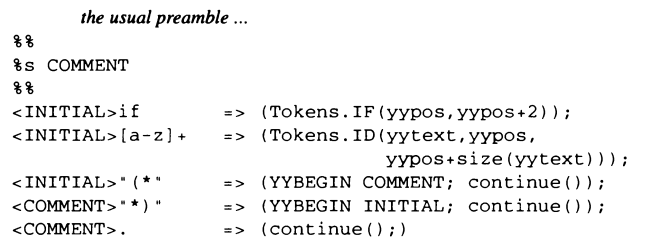
\includegraphics[width=.9\linewidth]{Lexical Analysis (2)/screenshot_2018-09-04_14-21-13.png}
\caption{\label{fig:org191c8da}
An example of explicity declaring startes}
\end{figure}

\section{Parsing (3)}
\label{sec:org766c1e8}
\subsection{Context-Free Grammars}
\label{sec:org5f16f00}
\begin{center}
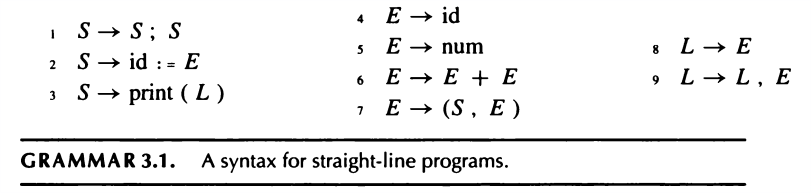
\includegraphics[width=.9\linewidth]{Parsing (3)/screenshot_2018-09-10_16-50-07.png}
\label{orgb873eb7}
\end{center}

\begin{itemize}
\item Parsers must read not only terminal symbols such as \texttt{+}, \texttt{-}, \texttt{num} and so on, but also the end-of-file marker
\begin{itemize}
\item \texttt{\$} is used to represent the end of file
\end{itemize}
\end{itemize}

\subsection{Predictive Parsing}
\label{sec:org38d69ed}
\subsubsection{General}
\label{sec:orgb0e942e}
\begin{itemize}
\item Some grammars are easy to parse using an algorithm known as \emph{recursive descent}
\begin{itemize}
\item Each grammar production turns into one clause of a recursive function
\item Works only on grammars where the first terminal symbol of each sub-expression provides enough information to choose which production to use
\item The advantage of this is that it can be constructed by hand without the need for automatic tools
\end{itemize}
\end{itemize}

\subsubsection{First And Follow Sets}
\label{sec:orgfae6a50}
\begin{itemize}
\item Given a string \(\gamma\) of terminal and nonterminal symbols, FIRST(\(\gamma\)) is the set of all terminal symbols that can begin any string derived from \(\gamma\)
\begin{itemize}
\item If two different productions \(X \to \gamma_1\) and \(X \to \gamma_2\) has overlapping FIRST sets the grammar cannot be parsed using predictive parsing
\end{itemize}

\item With respect to a particular grammar, given a string \(\gamma\) of terminals and nonterminals
\begin{itemize}
\item nullable(\(X\)) is true if \(X\) can derive the empty string
\item FIRST(\(\gamma\)) is the set of terminals that can begin strings derived from \(\gamma\)
\item FOLLOW(\(X\)) is the set of terminals that can immediately follow X
\begin{itemize}
\item That is \(t \in \text{FOLLOW} (X)\) if there is any derivation containing \(Xt\)
\end{itemize}
\end{itemize}

\item The following is true for the FIRST relation to strings of symbols
\begin{itemize}
\item \(\text{FIRST}(X\gamma) = \text{FIRST}[X\gamma]\) if not nullable\([X]\)
\item \(\text{FIRST}(X\gamma) = \text{FIRST}[X] \cup \text{FIRST}(\gamma)\) if not nullable\([X]\)
\end{itemize}
\end{itemize}

\subsubsection{Constructing a predictive parser}
\label{sec:org92ccf26}
\begin{center}
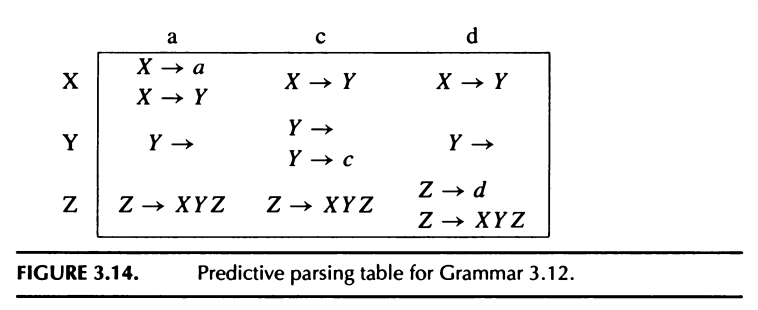
\includegraphics[width=.9\linewidth]{Parsing (3)/screenshot_2018-09-10_17-34-52.png}
\end{center}

\begin{itemize}
\item A predictive parsing table is a table that is indexed by nonterminals \(X\) and terminals \(T\)
\begin{itemize}
\item Constructed by entering a production \(X \to \gamma\) in row \(X\), column \(T\) of the table for each \(T \in \text{FIRST}(\gamma)\)
\item If \(\gamma\) is nullable enter the production in row \(X\), column \(R\) for each \(T \in \text{FOLLOW}[X]\)
\item If one of the entries contain more than one production predictive parsing will not work on the grammar
\item Grammars whose predictive parsing table tables contain no duplicate entries are called \(\text{LL}(1)\)
\end{itemize}

\item \(LL(k)\) parsing tables is a table whose rows and columns are every sequence of \(k\) terminals
\begin{itemize}
\item Rarely used in done, because the of the large tables
\end{itemize}

\item Grammars parsable with \(LL(k)\) parsing tables are called \(LL(k)\) grammars
\begin{itemize}
\item Any \(LL(k-1)\) grammar is also a \(LL(k)\) grammar
\end{itemize}
\end{itemize}

\subsubsection{Error recovery}
\label{sec:orgece4f7f}
\begin{itemize}
\item When during error recovery one must:
\begin{itemize}
\item Print out a meaning full message
\item Delete the thing causing the error to avoid running forever
\end{itemize}
\end{itemize}

\subsection{LR Parsing}
\label{sec:org36d552a}
\subsubsection{General}
\label{sec:org4f19358}
\begin{center}
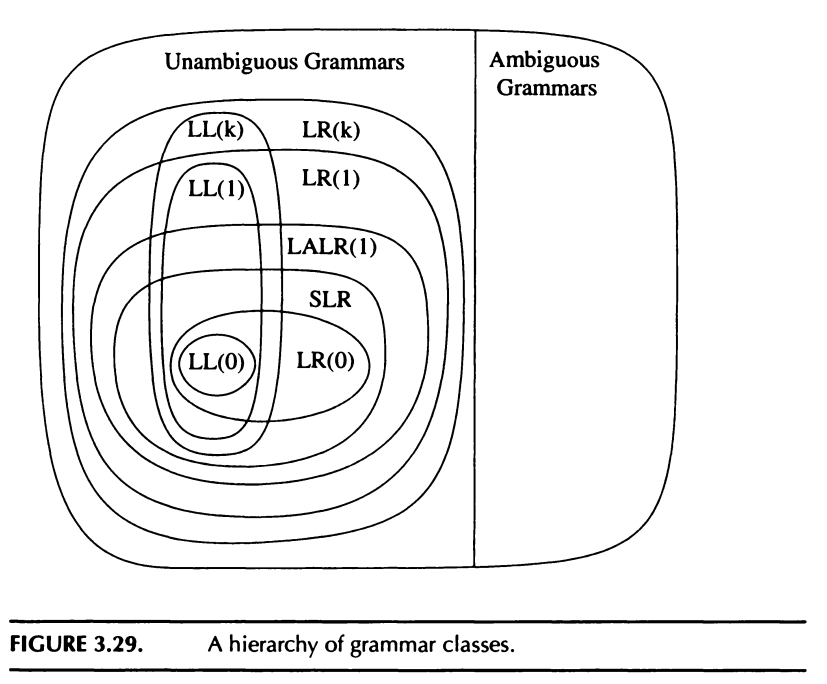
\includegraphics[width=.9\linewidth]{Parsing (3)/screenshot_2018-09-11_18-03-40.png}
\end{center}

\begin{itemize}
\item A powerfull technique for parsing is called \(\text{LR}(k)\) parsing
\begin{itemize}
\item It is able to postpone the decision until it has seen input tokens corresponding to the entire right-hand side of the production in question
\begin{itemize}
\item \(k\) more input tokens beyond
\end{itemize}
\end{itemize}

\item The parser has a stack and an input
\item The first \(k\) tokens of the input are the \textbf{lookahead}
\item Based on the contents of the stack and the lookahead the parser performs two kinds of actions
\begin{itemize}
\item \texttt{Shift}: move the first input token to the top of the stack
\item \texttt{Reduce}: Choose a grammar rule \(X \to A \ B \ C; \text{pop} \ C,B,A\)
\end{itemize}
\item The action of shifting the end-of-file marker \texttt{\$} is called \textbf{accepting} and cause the parser to stop successfully
\end{itemize}

\subsubsection{LR Parsing Engine}
\label{sec:orgf9a661c}
\begin{itemize}
\item The LR parser know when to shift and reduce by using a FA
\begin{itemize}
\item It is not applied to the input but to the stack
\item The edges are labeled by symbols that can appear on the stack
\end{itemize}
\end{itemize}

\begin{center}
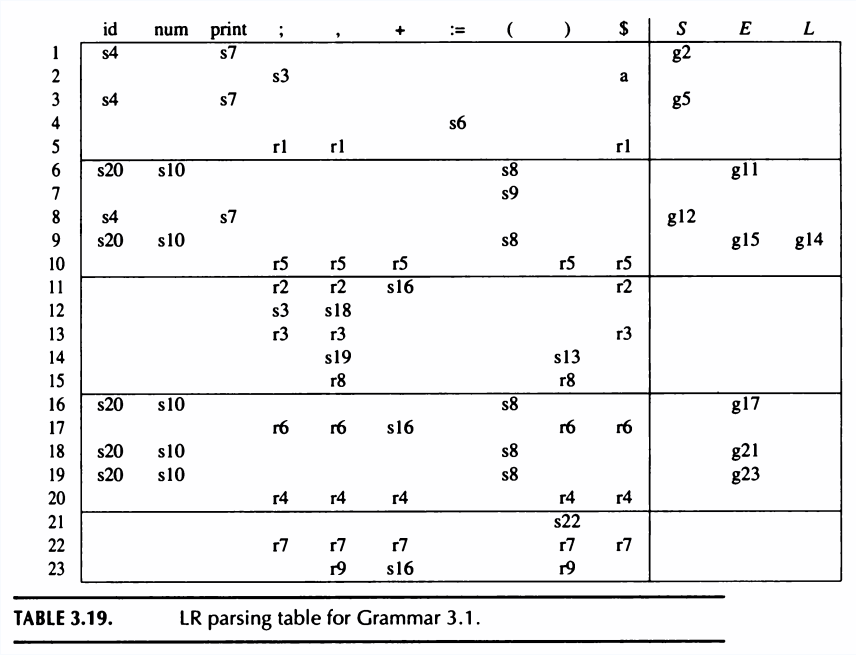
\includegraphics[width=.9\linewidth]{Parsing (3)/screenshot_2018-09-10_18-46-04.png}
\end{center}

\begin{itemize}
\item The elements in a transition table are labeled with four kinds of actions:
\begin{itemize}
\item \(\pmb sn\) Shift into state \(n\);
\item \(\pmb gn\) Goto state \(n\);
\item \(\pmb r k\) Reduce by rule \(k\);
\item \(\pmb a\) Accept;
\item Error is denote by a blank entry in the table
\end{itemize}

\item To use a transition table in parsing treat the shift and goto actions as edges of the DFA and scan the stack
\item Rather than rescan the stack again the parser can remember the state reached for each stack element.
\end{itemize}

\begin{figure}[htbp]
\centering
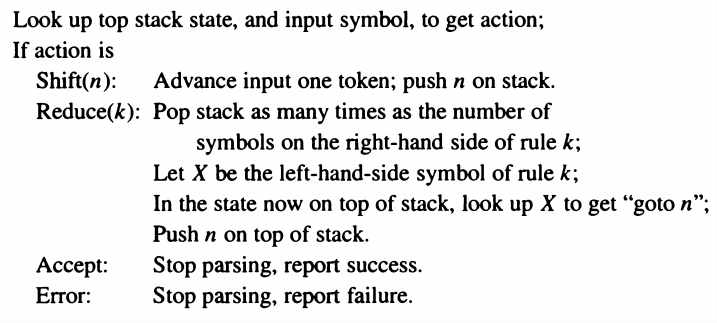
\includegraphics[width=.9\linewidth]{Parsing (3)/screenshot_2018-09-10_18-50-49.png}
\caption{\label{fig:org570caee}
The parsing algorithm}
\end{figure}

\subsubsection{\(LR(0)\) Parser generation}
\label{sec:org0cdfae0}
\begin{itemize}
\item An \(L(k)\) parser uses the contents of its stack and the next \(k\) tokens of the input to decide which action to take
\begin{itemize}
\item In practice \(k>1\) is not used for compilation
\item Grammars which has \(k=0\) is too weak to be very useful
\end{itemize}
\end{itemize}

\subsection{Using Parser Generators}
\label{sec:orgaacb1fe}
\subsubsection{ML-Yacc General}
\label{sec:orgcc8ac98}
\begin{figure}[htbp]
\centering
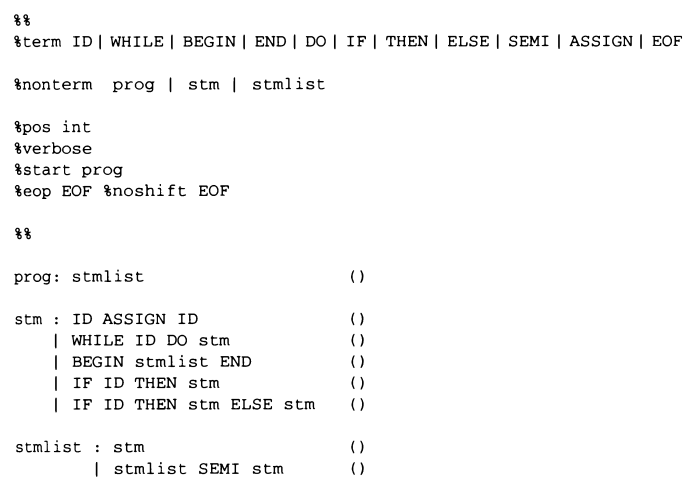
\includegraphics[width=.9\linewidth]{Parsing (3)/screenshot_2018-09-11_18-11-59.png}
\caption{\label{fig:orgf46531f}
Example of ML-Yacc without Semantic Actions}
\end{figure}

\begin{itemize}
\item ML-Yacc is a parser generator
\item An ML-Yacc specification is divided into three sections separated by \%\% marks
\end{itemize}
\begin{verbatim}
user declarations
%%
parser declarations
%% 
grammar rules
\end{verbatim}

\begin{itemize}
\item The \textbf{user declarations} are ordinary ML declarations usable from the semantic actions in later sections
\item The \textbf{parser declarations} include a list of the terminal symbols nonterminals and so on
\item The \textbf{grammars rules} are productions of the form
\end{itemize}
\begin{verbatim}
exp: exp plus exp (semantic action)
\end{verbatim}
\begin{itemize}
\item Where \texttt{exp} is a nonterminal producing a right hand side of \texttt{exp+exp} and \texttt{PLUS} is a terminal symbol
\begin{itemize}
\item The semantic action is written in ordinary ML and will be executed whenever the parser reduces using this rule
\end{itemize}
\end{itemize}

\subsubsection{Conflicts}
\label{sec:org9973bf2}
\begin{itemize}
\item ML-Yacc reports shift-reduce and reduce-reduce conflicts
\begin{itemize}
\item A \textbf{shift-reduce conflict} is a choice between shifting and reducing
\item A \textbf{reduce-reduce conflict} is a choice between reducing and reducing
\item By default ML-Yacc resolves shift-reduce conflicts by shifting and reduce-reduce conflicts by using the rule that appears earlier in the grammar
\end{itemize}

\item Most shift-reduce conflicts and reduce-reduce conflicts are serious problems and should be eliminated by rewriting the grammar
\end{itemize}

\subsubsection{Precedence Directives}
\label{sec:org7c0eb89}
\begin{itemize}
\item ML-Yacc has precedence directives to indicate the resolution of the class of \textbf{shift-reduce conflicts} that are caused by ambiguity in the grammar
\end{itemize}

\begin{figure}[htbp]
\centering
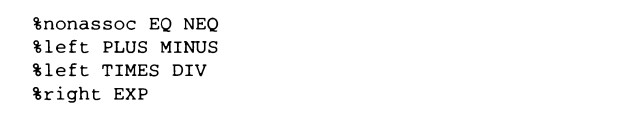
\includegraphics[width=.9\linewidth]{Parsing (3)/screenshot_2018-09-11_18-27-07.png}
\caption{\label{fig:org139f478}
Example of precedence directives that are used to indicate that + and - are left-assciative and bind equally tightly and that * and / are left-assciative and bind more tightly than +, that = \(\ne\) are nonassociative and binds more weekly than + and that \^{} is rightassociative and bind most tightly.}
\end{figure}

\subsubsection{Syntax Versus Semantics}
\label{sec:orgec63351}
\begin{itemize}
\item When given an identifier which can have multiple types e.g. numbers and booleans, one must change the grammar to make the two identifiers equal and let the semantic part of the compiler handle it
\end{itemize}

\subsection{Error Recovery}
\label{sec:org4d4181a}
\subsubsection{Recovery Using The Error Symbol}
\label{sec:orgbb18c25}
\begin{itemize}
\item Local error recovery mechanisms work by adjusting the parse stack and the inputs \emph{where the error was detected} in a way that will allow parsing to resume
\begin{itemize}
\item Many versions of the Yacc parser generator uses a special \emph{error} symbol to control the recovery process
\item Can be done by adding error-recovery productions
\end{itemize}

\item When the LR parser reaches an error state it does not following actions
\begin{enumerate}
\item Pop the stack (if necessary) until a state is reached in which the action for the \emph{error} token is \emph{shift}
\item Shift the \emph{error} token
\item Discard input symbols (if necessary) until a state is reached that has a non-error action on the current lookahead token
\item Resume normal parsing
\end{enumerate}
\end{itemize}

\subsubsection{Global Error Repair}
\label{sec:orgf7888c5}
\begin{itemize}
\item \textbf{Global error repair} finds the smallest set of insertions and deletions that would turn the source string into a syntactically correct string
\begin{itemize}
\item Even if the insertions and deletions are not at a point where an LL or LR parser would first report an error
\end{itemize}

\item \textbf{Burke-Fisher error repair:} Tries every possible single-token insertion, deletion or replacement at every point that occurs no earlier that \(K\) tokens before the point where the parser reported the error
\begin{itemize}
\item The correction that allows the parser to parse furthest past the original reported error is taken as the best error repair
\item Generally if a repair carries the parser \(R=4\) tokens beyond where it originally got stuck it is "good enough"
\item The advantage of this technique is that the grammar is not modified at all, nor are the parsing tables modified, only the parsing engine
\item The parsing engine must be able to back up \(K\) tokens and reparse
\begin{itemize}
\item Needs to remember what the parse stack looked like \(K\) tokens ago.
\item The algorithm maintains two parse stack the \emph{current} stack and the \emph{old} stack
\item Queue of \(K\) tokens is kept, as a new token is shifted it is pushed on the current stack and put onto the tail of the queue and the head is pooped
\end{itemize}
\end{itemize}

\item \textbf{Semantic actions:} Shift and reduce actions are tried repeatedly and discarded during the search for the best error repair
\begin{itemize}
\item The Burke-Fisher parser does not execute any of the semantic actions as the reductions are performed on the current stack
\begin{itemize}
\item Waits until the same reductions are performed on the \emph{old} stack
\end{itemize}
\end{itemize}

\item \textbf{Semantic value for insertions}: In repairing an error by insertion the parser needs to provide a semantic value for each token it inserts
\begin{itemize}
\item Done in ML-Yacc by using the \texttt{\%value} directive
\end{itemize}
\end{itemize}

\begin{figure}[htbp]
\centering
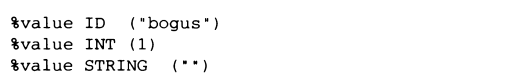
\includegraphics[width=.9\linewidth]{Parsing (3)/screenshot_2018-09-11_19-16-35.png}
\caption{\label{fig:org4bd403f}
Value directive example}
\end{figure}

\begin{itemize}
\item \textbf{Programmer-specified substitutions:} Some common kinds of errors cannot be repaired by the insertion or delection of a single token
\begin{itemize}
\item Should be tried first
\item In the ML-Yacc grammar specification the probrammer can use the \texttt{\%change} directive to suggest error corrections to be tried first, forfore the default "delete or insert each possible token" repairs
\end{itemize}
\end{itemize}

\begin{figure}[htbp]
\centering
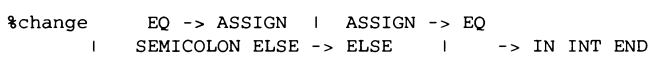
\includegraphics[width=.9\linewidth]{Parsing (3)/screenshot_2018-09-11_19-19-52.png}
\caption{\label{fig:org6816299}
Change directive example}
\end{figure}

\section{Abstract Syntax (4)}
\label{sec:org21547af}
\subsection{Semantic Actions}
\label{sec:orgb100ce7}
\begin{itemize}
\item For a rule \(A \to B \ C \ D\), the semantic action must return a value whose type is the one associated the nonterminal \(A\)
\begin{itemize}
\item It can build this value from the values associated with the matched terminals and nonterminal \(B,C,D\)
\end{itemize}

\item In a recursive-descent parser, the semantic actions are the values returned by the parsing functions, or the side effects of those functions, or both
\end{itemize}

\begin{figure}[htbp]
\centering
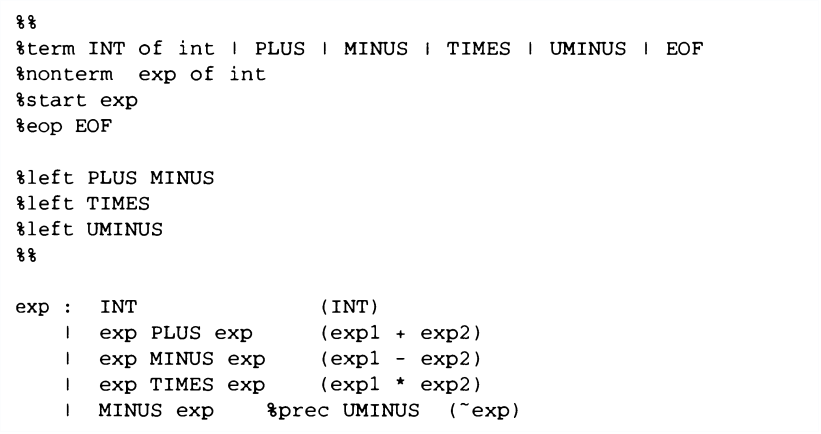
\includegraphics[width=.9\linewidth]{Abstract Syntax (4)/screenshot_2018-09-12_20-37-16.png}
\caption{\label{fig:org0276bc0}
ML-Yacc grammar with semantic actions}
\end{figure}

\begin{itemize}
\item A parser specification for ML-Yacc consists of a set of grammar rules each annotated with a semantic action that is an ML expression
\begin{itemize}
\item When ever the generated parser reduces by a rule it will execute the corresponding semantic action fragment
\item The semantic rules can refer to the semantic value of right-hand-side symbols
\item The value produced by every semantic expression must match the nonterminal
\item Implement semantic values by keeping a stack of them parallel to the state stack
\begin{itemize}
\item Where each symbol would be on a simple parsing stack the now is a semantic value
\end{itemize}
\end{itemize}
\end{itemize}

\begin{center}
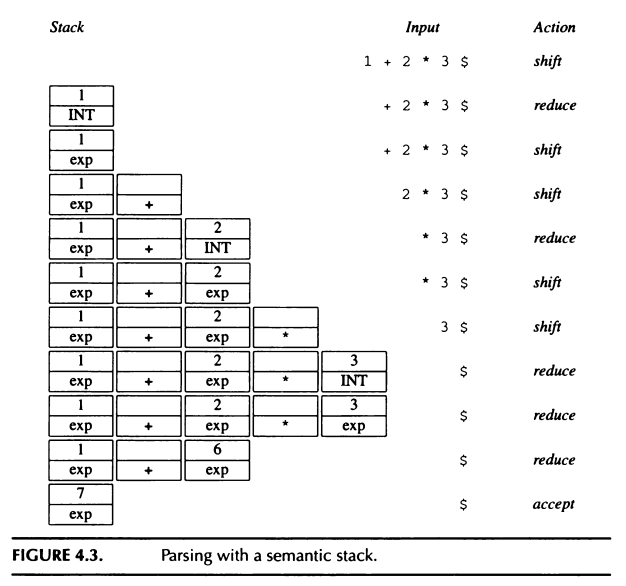
\includegraphics[width=.9\linewidth]{Abstract Syntax (4)/screenshot_2018-09-12_20-44-49.png}
\end{center}

\subsection{Abstract Parse Trees}
\label{sec:org59e4924}
\begin{center}
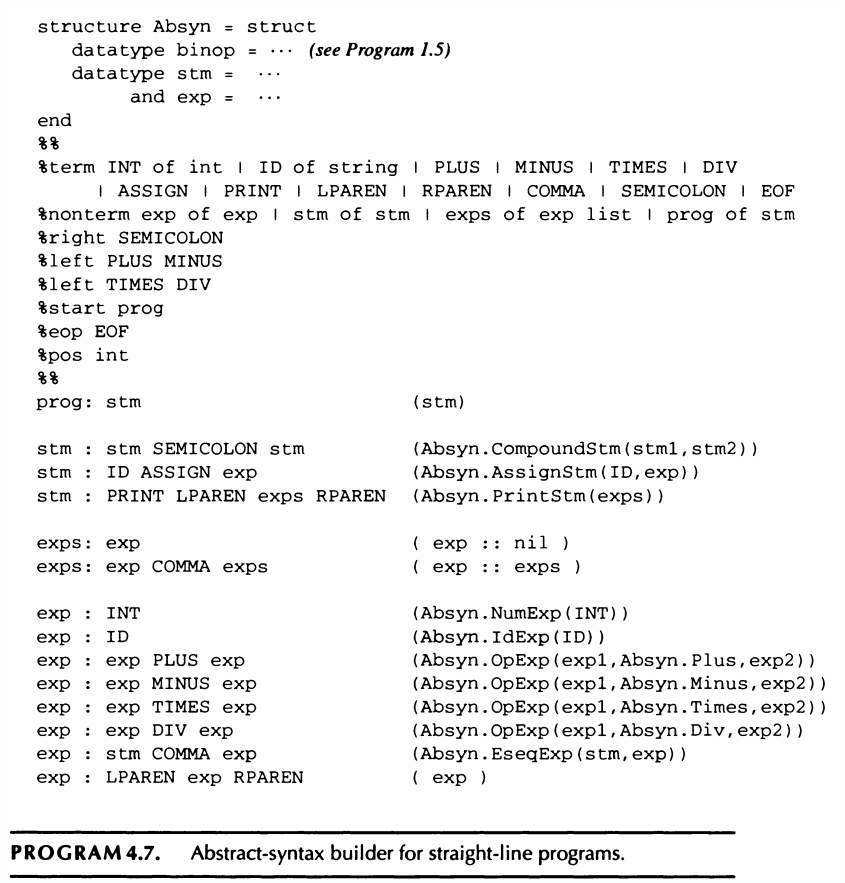
\includegraphics[width=.9\linewidth]{Abstract Syntax (4)/screenshot_2018-09-12_21-05-30.png}
\end{center}

\begin{itemize}
\item A way to separate the issues of parsing from the issues of semantics is to produce a \textbf{parse tree}
\begin{itemize}
\item A data structure that later phases of the compiler can traverse
\item It has exactly one leaf for each token of the input and one internal node for each grammar rule reduced during phase
\begin{itemize}
\item Is called a \textbf{concrete parsing tree} for concrete syntax
\item Is inconvenient to use directly
\item Depends too much on the grammar
\end{itemize}
\end{itemize}

\item An \textbf{abstract syntax} makes a clean interface between the parser and the later phases of the compiler
\begin{itemize}
\item The compiler will need to represent and manipulate abstract syntax trees as data structures (in ML using \texttt{datatype})
\end{itemize}

\item Since a grammar using abstract syntax tree often separates the different compiler operations one need to remember the position for reporting failures
\begin{itemize}
\item To remember positions accurately the abstract-syntax data structures must be sprinkled with \texttt{pos} fields
\item The ML-Yacc parser makes the beginning and end positions of each token available to the parser
\end{itemize}
\end{itemize}

\section{Semantic Analysis (5)}
\label{sec:orgec2f3e2}
\subsection{General}
\label{sec:org605b567}
\begin{itemize}
\item The \textbf{semantic analysis} phase of a compiler
\begin{itemize}
\item connects variable definitions to their uses
\item checks that each expression has a correct type
\item translates the abstract syntax into a simpler representation suitable for generating machine code
\end{itemize}
\end{itemize}

\subsection{Symbol Tables}
\label{sec:org330b9d3}
\subsubsection{General}
\label{sec:org8abf1a1}
\begin{itemize}
\item This phase is characterized by the maintenance of \textbf{symbol tables} mapping identifiers to their types and locations 
\begin{itemize}
\item Also called \textbf{environments}
\item As the declarations of types, variables and functions are processed, these identifiers are bound to "meanings" in the symbol tables
\item When \textbf{uses} (non-defining occurrences) of identifiers are found, they are looked up in the symbol tables
\item Each local variable in a program has a scope in which it is visible
\begin{itemize}
\item As the semantic analysis reaches the end of each scope, the identifier bindings local to that scope are discarded
\end{itemize}
\end{itemize}

\item An \textbf{environment} is a set of bindings
\begin{itemize}
\item Denoted by the \(\mapsto\) arrow
\item e.g. an environment \(\sigma_0\) which contains the bindings \(\{g \mapsto \text{string}, a \mapsto \text{int}\}\) meaning that \(a\) is an integer variable and \(g\) is a string variable
\item When two environments are added the new variables, i.e. the left hand side, has precedence over the existing types
\item Can be implemented in to ways
\begin{itemize}
\item \textbf{Functional style:} where the original environment are kept in pristine condition
\item \textbf{Imperative style:} where the environment is modified to become a new environment and a undo stack is kept
\end{itemize}
\end{itemize}

\item In some languages there can be several active environments at once
\begin{itemize}
\item Each module or class or record in the program has a symbol table \(\sigma\) of its own
\end{itemize}
\end{itemize}

\subsubsection{Efficient Imperative Symbol Tables}
\label{sec:orgcb0fd90}
\begin{center}
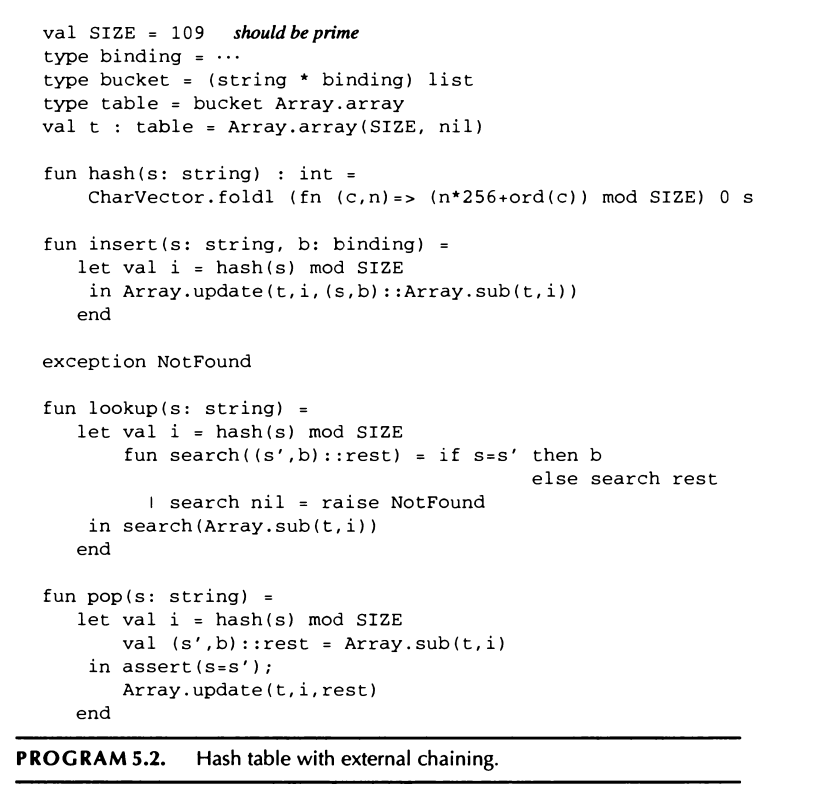
\includegraphics[width=.9\linewidth]{Semantic Analysis (5)/screenshot_2018-09-16_18-28-18.png}
\end{center}

\begin{itemize}
\item Because a large program may contain thousands of distinct identifiers symbol tables must permit efficient lookup
\begin{itemize}
\item Imperative-style environments are usually implemented using hash table, which are very efficient
\item The operation \(\sigma' = \sigma + \{a \mapsto \tau \}\) is implemented by inserting \(\tau\) in the hash table with key \(a\)
\item A simple \textbf{hash table with external chaining} works well and supports deletion easily
\begin{itemize}
\item When we will need to delete \(\{a \mapsto \tau \}\) to recover \(\sigma\) at the end of the scope of \(a\)
\end{itemize}
\end{itemize}
\end{itemize}

\subsubsection{Efficient Functional Symbol Tables}
\label{sec:orgd6fce72}
\begin{itemize}
\item In the functional style, we wish to compute \(\sigma' = \sigma + \{a \mapsto \tau\}\) in such a way that we still have \(\sigma\) available to look up identifiers
\begin{itemize}
\item Instead of altering a table we create a new table by computing the "sum" of an existing table and a new binding
\item By using binary search tree we can perform functional additions to search trees efficiently
\end{itemize}
\end{itemize}

\section{Activation Records (6)}
\label{sec:orgf3253fe}
\subsection{Higher order functions}
\label{sec:orgd986a56}
\begin{itemize}
\item In some languages such as C the local variables are destroyed when a function returns
\item In languages supporting both nested functions and function valued variables, it may be necessary to keep local variables after a function has returned
\begin{itemize}
\item It is the combination of nested functions and functions returned as results that cause the local variables to have longer lifetimes than their enclosing function invocations
\item Pascal (and Tiger) has nested functions but do not have functions as return variables, C has functions as returnable variables but not nested functions
\begin{itemize}
\item These languages can use stacks to hold local variables
\end{itemize}
\item ML, Scheme and several other languages have both nested functions and functions as returnable values
\begin{itemize}
\item This combination is called higher-order functions
\item They cannot use a stack to hold all local variables
\end{itemize}
\end{itemize}
\end{itemize}

\subsection{Stack Frames}
\label{sec:orgc2b04a0}
\begin{center}
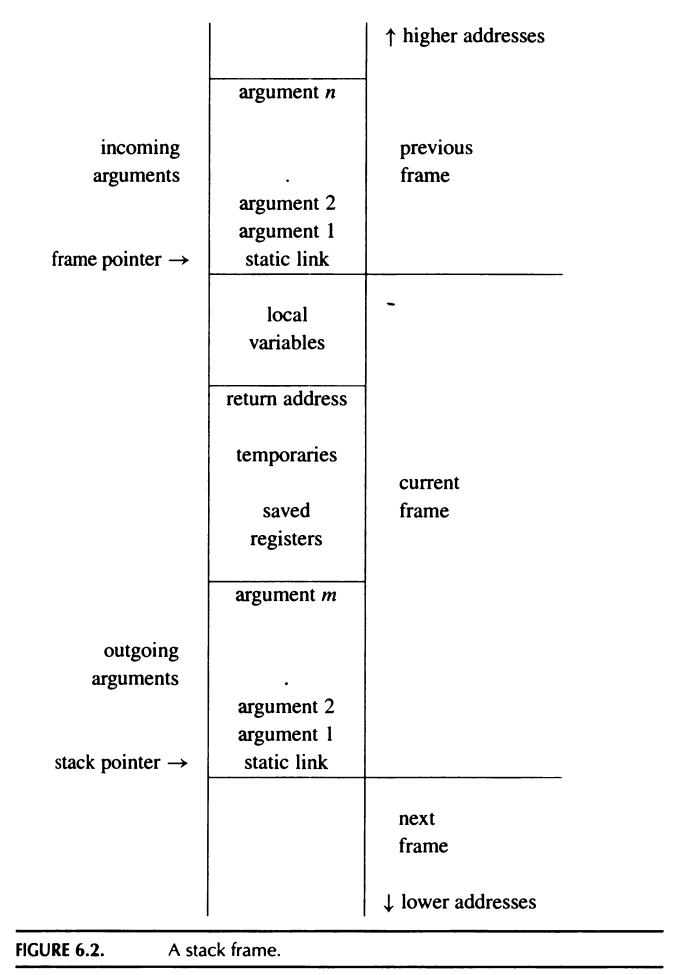
\includegraphics[width=.9\linewidth]{Activation Records (6)/screenshot_2018-10-22_16-44-34.png}
\end{center}

\subsubsection{General}
\label{sec:org0994ae9}
\begin{itemize}
\item Since we need to push and pop in large batches and access variables deep within the stack the standard stack is not suitable for storing local variables
\item The stack is treated as a big array with a special register, the \emph{stack pointer} that points to some location
\begin{itemize}
\item All locations beyond the stack pointer are considered \textbf{garbage}
\item All locations before the stack pointer are considered \textbf{allocated}
\item It usually grows only at the entry to a function, by an increment large enough to hold all the variables for that function
\begin{itemize}
\item It shrinks at by the same amount when exiting the function
\end{itemize}
\item The area on the stack devoted to the local variables, parameters, return address and other temporaries for a function is called the functions \textbf{activation record} or \textbf{stack frame}
\item Run-time stacks usually start at a high memory address and grow toward smaller addresses
\item The design of the frame layout takes into account the particular features of an instruction set architecture and the programming language being compiled
\begin{itemize}
\item A manufacture of a computer often prescribes a "standard" frame layout to be used on that architecture where possible by all compilers for all programming languages
\item By using the standard layout we gain the considerable benefit that functions written in one language can call functions written in another language
\end{itemize}
\item The \emph{return address} is created by the \texttt{CALL} instruction and tells where control should return upon completion of the current function
\item Some local variables are kept in the frame others are kept in machine registers
\begin{itemize}
\item Sometimes a local variable kept in the registers needs to be saved into the frame to make room for other uses of the register
\item There is an area in the frame for this purpose
\end{itemize}
\item When the current function calls other functions it can use the \emph{outgoing argument} space to parse parameters
\end{itemize}
\end{itemize}

\subsubsection{The frame pointer}
\label{sec:org1051c5b}
\begin{itemize}
\item If a function \(g(\dots)\) calls the function \(f(a_1, \dots,a_n)\) we say \(g\) is the caller and \(f\) is the callee
\begin{itemize}
\item On entry to \(f\) the stack pointer points to the first argument that \(g\) passes to \(f\)
\item On entry, \(f\) allocates a frame by simply subtracting the frame size from the stack pointer
\begin{itemize}
\item The old \texttt{SP} becomes the current frame pointer \texttt{FB}
\end{itemize}
\item In some frame layouts \texttt{FP} is a separate register
\begin{itemize}
\item The old value of \texttt{FP} is saved in memory
\item The new \texttt{FP} becomes the old \texttt{SP}
\item When \(f\) exits it just copies \texttt{FP} back to \texttt{SP} and fetches back the save \texttt{FP}
\item This is useful if the frame size can vary or if frames are not always continuous on the stack
\end{itemize}
\item If the frame size is fixed it is not necessary to use a register for \texttt{FP} at all
\begin{itemize}
\item For each function \(f\) the \texttt{FP} will always differ from \texttt{SP} by some fixed amount
\item \texttt{FP} is a "fictional" register whose value is always \texttt{SP} + \emph{framesize}
\end{itemize}
\item Since the frame size is not know until quite late in the compilation process
\begin{itemize}
\item Therefore it is convenient to talk about a frame pointer
\item Also since we put the formals and locals right near the frame pointer at offsets that are known early
\item Temporaries and saved registers go farther away at offsets that are known later
\end{itemize}
\end{itemize}
\end{itemize}

\subsubsection{Registers}
\label{sec:org9080cb4}
\begin{itemize}
\item A modern machine has a large set of registers
\begin{itemize}
\item To make compile programs run fast, it's useful to keep local variables, intermediate results of expressions and other values in registers instead of in the stack frame
\item Registers can be directly accessed by arithmetic instruction
\begin{itemize}
\item On most machines it requires separate \emph{load} and \emph{store} instructions
\item Even on machines whose arithmetic instructions can access memory it is faster to access registers
\end{itemize}
\end{itemize}

\item A machine usually has only one set of registers but many different procedures and functions need to use registers
\begin{itemize}
\item If a function \(f\) is using register \(r\) to hold a local variable and calls procedure \(g\) which also uses \(r\) for its own calculations
\begin{itemize}
\item Then one must save \(r\) into the stack frame before \(g\) uses it
\item Both \(f\) and \(g\) could have that responsibility
\end{itemize}
\item \(r\) is a \textbf{caller-save} register if the caller must save and restore the register
\item \(r\) is a \textbf{callee-save} register if the callee must save and restore the register
\item On most machine architecture the notion of caller-save and callee-save registers is not something built into the hardware but it is a convention described in the machine's reference manual
\item Some times saves and restores are unnecessary
\begin{itemize}
\item e.g. if the caller knows a variable will no be needed by the callee
\end{itemize}
\item One will rely on our register allocator to choose the appropriate kind of register for each variable and temporary value
\end{itemize}
\end{itemize}

\subsubsection{Parameter Passing}
\label{sec:org0ba1617}
\begin{itemize}
\item In the calling conversions for machines that where designed in the 1970s the arguments where passed on the stack
\item Since most functions use less than four arguments some of the arguments are typically passed through the registers
\begin{itemize}
\item It specifies that the first \(k\) arguments (typically 4 or 6) of a function are passed in register \(r_p, \dots, r_{p+k-1}\) and the rest are passed in memory
\item If \(f(a_1, \dots, a_n)\) calls \(h(z)\) it must pass the argument \(z\) in \(r_1\) so \(f\) saves the old contents of \(r_1\) (the value \(a_1\)) become calling \(h\)
\end{itemize}

\item The reasons passing argument in registers saves time is
\begin{enumerate}
\item Some procedure don't call other procedures
\begin{itemize}
\item They are called \textbf{leaf} procedures
\item Leaf procedures needs not write their incoming arguments to memory
\item They do not need to allocate a stack frame at all
\end{itemize}
\item Some optimizing compilers use \emph{interprocedural register allocation}
\begin{itemize}
\item It analyses all functions in an entire program at once
\item They assign difference procedures different register in which to receive parameters and hold local variables
\end{itemize}
\item Even if \(f\) is not a leaf procedure it might be finished with all its use of argument \(x\) by the time it calls \(h\)
\begin{itemize}
\item \(f\) can overwrite \(r_1\) without saving it
\end{itemize}
\item Some architecture have \emph{register windows}
\begin{itemize}
\item Each function invocation can allocate a fresh set of registers without memory traffic
\end{itemize}
\end{enumerate}

\item \(f\) needs to write an incoming parameter into the frame 
\begin{itemize}
\item Ideally its frame layout should matter only in the implementation of \(f\)
\item A straightforward approach would be for the caller to pass argument \(a_1, \dots, a_k\) in registers and \(a_{k+1}, \dots, a_n\) at the end of its own frame
\item In the standard calling convention of many modern machines the calling function reserves space for the register arguments in its own frame next to the place where it writes argument \(k+1\)
\begin{itemize}
\item The caller does no write anything there
\item The space is written into by the called function
\end{itemize}
\item Another way is to take the address of a local variable and use \emph{call-by-reference}
\begin{itemize}
\item The programmer does not explicitly manipulate the address of a variable \(x\)
\item If \(x\) is passed as the argument to \(f(y)\) where \(y\) is a "by reference" parameter the compiler generates code to pass the address of \(x\) instead of the contents of \(x\)
\end{itemize}
\end{itemize}
\end{itemize}

\subsubsection{Return Addresses}
\label{sec:org70b4e2f}
\begin{itemize}
\item When a function \(g\) calls \(f\), eventually \(f\) must return
\begin{itemize}
\item It needs to know where to go back to
\item If the call instruction within \(g\) is at address \(a\) then (usually) the right place to return to is \(a+1\)
\begin{itemize}
\item This is called the return address
\end{itemize}
\item On some old machines the return address was pushed on the stack by the call instruction
\item Modern science has shown that it is faster and more flexible to pass the return address in a register
\item On modern machine the \emph{call} instruction merely puts the return address in a designated register
\begin{itemize}
\item On non leaf procedure would have to write it to the stack
\end{itemize}
\end{itemize}
\end{itemize}

\subsubsection{Frame Resident Variables}
\label{sec:orgd866d8f}
\begin{itemize}
\item Values are only written to memory for one of these reasons
\begin{itemize}
\item The variable will be passed by reference, so it must have a memory address
\item The variable is accessed by a procedure nested inside the current one
\item The value is too big to fit into a single register
\item The variable is an array, for which address arithmetic is necessary to extract components
\item The register holding the variable is needed for a specific purpose
\begin{itemize}
\item e.g parameter passing
\item may be moved by the compiler to other registers instead of storing them in memory
\end{itemize}
\item There are so many local variables and temporary values that they won't all fit in registers
\begin{itemize}
\item Some of them are "spilled into the frame"
\end{itemize}
\end{itemize}

\item A variable \textbf{escapes} if it is passed by reference, its address taken or it is accessed from a nested function
\item When a formal parameter or local variable is declared it's convenient to assign it a location either in registers or in the stack frame, right at that point in processing the program
\begin{itemize}
\item The occurrences of that variable are translated into machine code that refers to the right locations
\item A good compiler must assign provisional location to all formals and locals and decide later which of them should really go in registers
\end{itemize}
\end{itemize}

\subsubsection{Static Links}
\label{sec:org70494ed}
\begin{itemize}
\item In languages that allow nested function declarations (e.g. ML and Tiger) the inner functions may use variable declared in outer functions which is called a \textbf{block structure}
\item To accomplish at block structure there are several methods
\begin{itemize}
\item Whenever a function \(f\) is called it can be passed a pointer to the frame of the function statically enclosing \(f\)
\begin{itemize}
\item Called a static link
\item In each procedure call or variable access, a chain of zero or more fetches is required
\end{itemize}
\item A global array can be maintained containing in position \(i\) a pointer to the frame of the most recently entered procedure whose static nesting depth is \(i\)
\begin{itemize}
\item Called a \textbf{display}
\end{itemize}
\item When \(g\) calls \(f\), each variable of \(g\) that is actually accessed by \(f\) is passed to \(f\) as an extra argument
\begin{itemize}
\item Called lambda lifting
\end{itemize}
\end{itemize}
\end{itemize}

\section{Liveness Analysis (10)}
\label{sec:org111178d}
\subsection{General}
\label{sec:org2a41f71}
\begin{center}
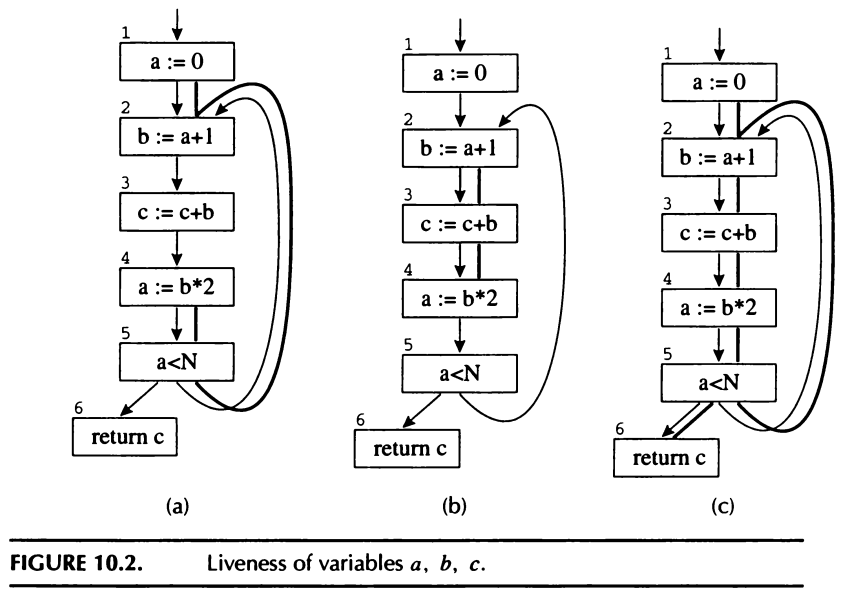
\includegraphics[width=.9\linewidth]{Liveness Analysis (10)/screenshot_2018-11-19_07-46-24.png}
\end{center}

\begin{itemize}
\item To decide which registers are safe to use a \textbf{liveness analysis} is performed on the IR  
\begin{itemize}
\item We say that a variable is \textbf{live} is it holds a value that may be needed in the future
\item A control flow graph is often used
\end{itemize}
\end{itemize}

\subsection{Solution of Dataflow Equations}
\label{sec:orgcf3c395}
\subsubsection{Terminology}
\label{sec:org3d9b2ce}
\begin{itemize}
\item Determining the live range of each variable is an example of a \textbf{dataflow} problem

\item A flow-graph node has
\begin{itemize}
\item \textbf{out-edges} that lead to \textbf{successor} nodes
\item \textbf{in-edges} that come from \textbf{predecessor} nodes
\item the set \(pred[n]\) is all the predecessor of node \(n\)
\item the set \(succ[n]\) that is all successors of node \(n\)
\end{itemize}

\item An assignment to a variable or temporary \textbf{defines} that variable
\begin{itemize}
\item An occurrence of a variable on the right-hand side of an assignment or other expressions \textbf{uses} that variable
\item The \(def\) of a variable is the set of graph nodes that define it
\item The \(def\) of the graph node is the set of variables that it defines
\item The \(use\) of a variable is the set of graph nodes that uses it
\item The \(use\) of the graph node is the set of variables that it uses
\end{itemize}

\item A variable is \textbf{live} on an edge if there is a directed path from the edge to a \emph{use} of that variable that does not flow through any \emph{def}
\begin{itemize}
\item A variable is \textbf{live-in} a node if it is live on any of the in-edges of that node
\item A variable is \textbf{live-out} a node if it is live on any of the out-edges of that node
\end{itemize}
\end{itemize}

\subsubsection{Calculation of Liveness}
\label{sec:org4dcba7a}
\begin{center}
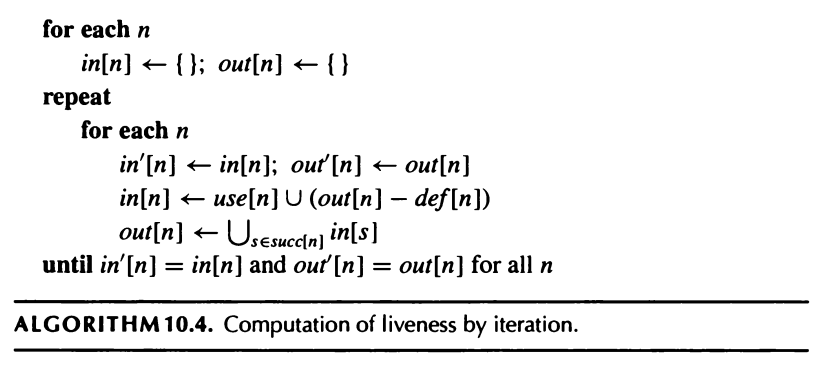
\includegraphics[width=.9\linewidth]{Liveness Analysis (10)/screenshot_2018-11-19_08-04-47.png}
\end{center}
\begin{itemize}
\item Liveness information can be calculated from \emph{use} and \emph{def} as follows
\begin{enumerate}
\item If a variable is in \(use[n]\) the it is \emph{live-in} at node \(n\)
\begin{itemize}
\item If the statements uses a variable the variable is live on entry to that statement
\end{itemize}
\item If a variable is \emph{live-in} at node \(n\), then it is \emph{live-out} at all nodes \(m\) in \(pred[n]\)
\item If a variable is \emph{live-out} in node \(n\), and not in \(def[n]\), then the variable is also \emph{live-in} at \(n\)
\begin{itemize}
\item If someone needs the value of \(a\) at the end of statement \(n\) and \(n\) does not provide that value, then \(a\)'s value is needed even on entry to \(n\)
\end{itemize}
\end{enumerate}

\item Flow-graph nodes that only have one predecessor and one successor are not very interesting
\begin{itemize}
\item They can be merged with their predecessor and successors
\item This results in a graph with fewer nodes
\item Faster running time
\end{itemize}

\item It can be practical to compute dataflow for one variable at a time as information for that variable is needed
\begin{itemize}
\item This would mean repeating the dataflow traversal once for each temporary
\item Starting from each \emph{use} site of a temporary \(t\) and tracing backward using depth-first search
\item The search stops at definition of the temporary
\item Many temporaries have short live range and the searches would terminate quickly
\end{itemize}
\end{itemize}

\subsubsection{Representation of Sets}
\label{sec:org340d9e2}
\begin{itemize}
\item There are two good ways to represent sets for data flow equations
\begin{enumerate}
\item As arrays of bits
\begin{itemize}
\item If there are \(N\) variables in the program, the bit-array representation uses \(N\) bits for each set
\item Calculating the union of two sets is done by or-ring the corresponding bits at each positionn
\item It takes \(N/K\) operations if there is \(K\) bits
\end{itemize}
\item As sorted list of variables
\begin{itemize}
\item Represented as a linked list of its members, sorted by any totally ordered key e.g. variable name
\item Calculating the union is done by merging the list
\item It takes time proposition to the size of the sets being unioned
\end{itemize}
\end{enumerate}

\item When the sets (fewer than \(N/K\) elements the sorted-list representation is asymptotically faster
\item When the sets are dense the bit-array representation is better
\end{itemize}

\subsubsection{Time Complexity}
\label{sec:org16e65cb}
\begin{itemize}
\item The worst case running time of the algorithm is \(O(N^4 )\)
\begin{itemize}
\item Ordering the nodes using depth-first-search usually bring the number of iteration down to two or three with an algorithm that runs between \(O(N)\) and \(O(N^2)\) is practice
\end{itemize}
\end{itemize}

\subsubsection{Least Fixed Points}
\label{sec:orgad74afa}
\begin{itemize}
\item Any solution to the dataflow equations is a \emph{conservative approximation}
\begin{itemize}
\item It can be assured that if \(a\) is needed at some node \(n\) then it can be assured that \(a\) is live-out at node \(n\) in any solution to the equations
\item We might calculate that \(d\) is live-out but it doesn't mean its value is really used
\end{itemize}

\item \textbf{Theorem.} Equations 10.3 have more than one solution
\item \textbf{Theorem.} If \(in_X[n]\) and \(in_Y[n]\) are the live-in sets for some node \(n\) in solution \(X\) and \(Y\), then \(in_X[n] \subseteq in_Y[n]\)

\item Algorithm 10.4 always computes the least fixed points
\end{itemize}

\subsubsection{Static vs. Dynamic Liveness}
\label{sec:org7a1cc41}
\begin{itemize}
\item \textbf{Theorem.} There is no program \(H\) that takes as input any program \(P\) and input \(X\) and (without infinite-looping) returns true if \(P(X)\) halts and false if \(P(X)\) infinite loops
\item \textbf{Corollary.} No program \(H'(X,L)\) can tell, for any program \(X\) and label \(L\) within \(X\) whether the label \(L\) is ever reached on an execution of \(X\)
\item Because of the halting problem there does not exists any general algorithm that can tell if a variable is truly need in a specific place at run time
\item \textbf{Dynamic liveness} A variable \(a\) is dynamically live at node \(n\) if some execution of the program goes from \(n\) to a use of \(a\) without going through any definition of \(a\)
\item \textbf{Static liveness} A variable \(a\) is statically live at node \(n\) if there is some path of control-flow edges from \(n\) to some use of \(a\) that does not go through a definition of \(a\)
\end{itemize}

\subsubsection{Interference Graphs}
\label{sec:org4be51b7}
1\begin{center}
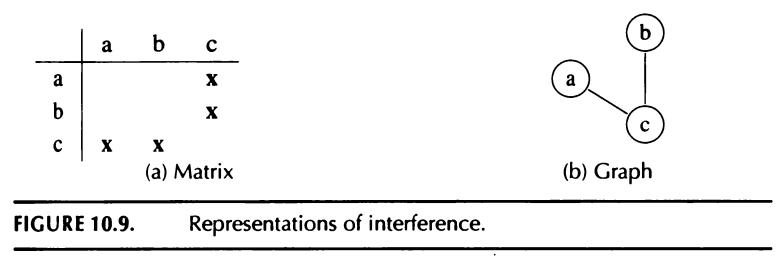
\includegraphics[width=.9\linewidth]{Liveness Analysis (10)/screenshot_2018-11-19_10-14-34.png}
\end{center}

\begin{itemize}
\item Liveness information is used for several kinds of optimization in a compiler
\begin{itemize}
\item For some optimizations we need to know which variables are live at each node in the flow graph
\end{itemize}

\item One of the most important applications of liveness analysis is for register allocation
\begin{itemize}
\item We have a set of temporaries \(a,b,c,\dots\) that must be allocated to registers \(r_1,\dots,r_k\)
\item A condition that prevents \(a\) and \(b\) being allocated to the same register is called an \textbf{interference}
\item The most common kind of interference is caused by overlapping live ranges when \(a\) and \(b\) are both live at the same program point
\begin{itemize}
\item Then they cannot be put in the same register
\item There are other causes e.g. when \(a\) must be generated by an instruction that cannot address register \(r_1\) then \(a\) and \(r_1\) interfere
\end{itemize}
\end{itemize}

\item To add interference edges for each new definition considering a move instruction
\end{itemize}
\begin{center}
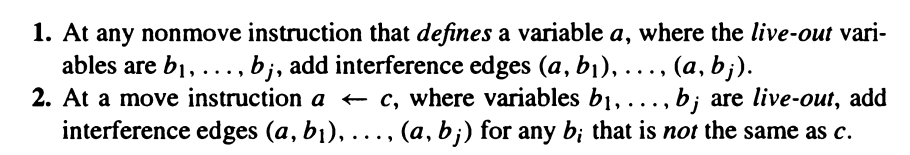
\includegraphics[width=.9\linewidth]{Liveness Analysis (10)/screenshot_2018-11-19_10-17-23.png}
\end{center}

\section{Register Allocation (11)}
\label{sec:orge6055d2}
\subsection{General}
\label{sec:org908baa5}
\begin{itemize}
\item The job of the register allocator is
\begin{itemize}
\item To assign the many temporaries to a small number of machine registers
\item Where possible to assign the source and destination of a \texttt{MOVE} to the same register e.g. deleting the \texttt{MOVE}
\end{itemize}

\item From an examination of the control and dataflow graph an \textbf{interference graph} can be derived
\begin{itemize}
\item Each node in the interference graph represents a temporary value
\item Each edge \((t_1,t_2)\) indicate a pair of temporaries that cannot be assigned to the same register
\end{itemize}

\item The interference graph is colored
\begin{itemize}
\item As few colors as possible should be used
\item No pair of nodes connected by an edge may be assigned the same color
\item The "colors" correspond to registers
\item If the target machine has \(K\) registers we can \(K\) color the graph
\begin{itemize}
\item Then coloring is a valid register assignment for the interference graph
\end{itemize}
\item If there is no \(K\) coloring some of variables and temporaries should be kept in memory instead
\begin{itemize}
\item This is called \textbf{spilling}
\end{itemize}
\end{itemize}
\end{itemize}

\subsection{Coloring by Simplification}
\label{sec:org5460ea4}
\begin{itemize}
\item Register allocation is an \emph{NP}-complete problem
\item Graph coloring is also \emph{NP}-complete

\item The following is a linear-time approximation algorithm with good results with the following phases
\begin{itemize}
\item \textbf{Build:} Construct the interference graph
\begin{itemize}
\item Dataflow analysis is used to compute the set of temporaries that are simultaneously live at each program point
\item We add an edge to the graph for each pair of temporaries in the set
\item Repeated for all program points
\end{itemize}

\item \textbf{Simplify:} The graph is colored using a simple heuristic
\begin{itemize}
\item \(K\) is the number of registers in the machine
\item Suppose the graph \(G\) contains a node \(m\) with fewer than \(K\) neighbors
\item Let \(G'\) be the graph \(G-\{m\}\) obtained by removing \(m\)
\item If \(G'\) can be colored. then so can \(G\)
\item This leads naturally to a stack-based/reserves algorithm for coloring
\begin{itemize}
\item We repeatedly remove nodes of degree less than \(K\)
\item Each simplification will decrease the degrees of other nodes
\end{itemize}
\end{itemize}

\item \textbf{Spill:} Suppose at some point during simplification the graph \(G\) has nodes only of significat degree, that is nodes of degree \(\geq K\)
\begin{itemize}
\item The simplify heuristic fail and we mark some node for spilling
\item We choose some node in the graph and decide to represent it in memory during program execution
\item An optimistic approximation to the effect of spilling is that the spilled node does not interfere with any of the other remaining in the graph
\item It can be removed the node and pushed on the stack as the simplify process continuous
\end{itemize}

\item \textbf{Select:} Colors are assigned to the nodes in the graph
\begin{itemize}
\item Starting with the empty graph
\item The original graph is rebuild by repeatedly adding a node from the top of the stack
\item When we add a node to the graph there must be a color for it
\item When potential spill node \(n\) that was pushed using the Spill heuristic is popped there is no guarantee that it will be colorable
\begin{itemize}
\item In this case we have an \textbf{actual spill}
\item No color is assigned and the Select phase is continued to identify other actual spils
\item If not we can color \(n\) which is known as \textbf{optimistic coloring}
\end{itemize}
\end{itemize}

\item \textbf{Start over:} If the \textbf{Select} phase is unable to find a color for some node(s) 
\begin{itemize}
\item The Program must be rewritten to fetch them from memory just before each use and store them back after each definition
\item A spilled temporary will turn into several new temporaries with tiny live range
\item These will interfere with other temporaries in the graph
\item The algorithm is repeated on this rewritten program
\item This process iterates until simplify succeeds with no spills
\begin{itemize}
\item Typically one or two iteration almost always suffice
\end{itemize}
\end{itemize}
\end{itemize}
\end{itemize}

\subsection{Coalescing}
\label{sec:org95e207b}
\subsubsection{Algorithm}
\label{sec:org0179ee4}
\begin{center}
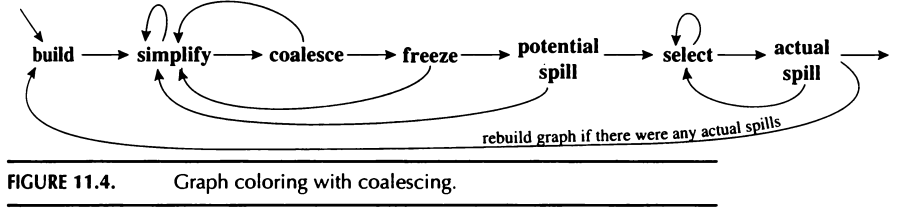
\includegraphics[width=.9\linewidth]{Register Allocation (11)/screenshot_2018-11-19_11-03-57.png}
\end{center}

\begin{itemize}
\item If there is no edge between the source and destination of a move instruction the move can be eliminated
\begin{itemize}
\item The source and destination nodes are \textbf{coalesced} into a new node whose edges are the union of those of the nodes being replaced
\item In principle any pair of nodes not connected by an interference edge could be coalesced
\item The node being introduced is more constrained than those being remove
\begin{itemize}
\item Since it contains a union of edges
\end{itemize}
\item Could make a \(K\) colorable graph no longer \(K\) colorable
\end{itemize}

\item Strategies to coalesce a graph that is safe which does not render the graph uncolorable 
\begin{itemize}
\item \textbf{Briggs:} Nodes \(a\) and \(b\) can be coalesced if the resulting node \(ab\) will have fewer than \(K\) neighbors of significant degree
\item \textbf{George:} Nodes \(a\) and \(b\) can be coalesced if, for every neighbor \(t\) of \(a\) either \(t\) already interferes with \(b\) or \(t\) is of insignificant degree
\end{itemize}

\item Phases of register allocator with coalescing
\end{itemize}
\begin{center}
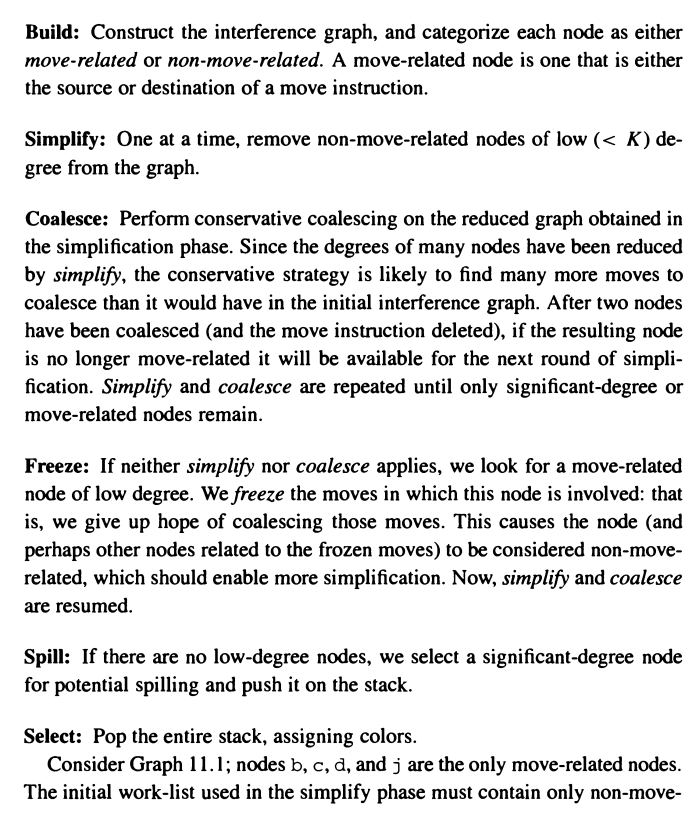
\includegraphics[width=.9\linewidth]{Register Allocation (11)/screenshot_2018-11-19_11-08-01.png}
\end{center}

\subsubsection{Spilling}
\label{sec:orgb960e55}
\begin{itemize}
\item If spilling is necessary build and simplify must repeated on the whole program
\begin{itemize}
\item The simplest version of the algorithm discards any coalescence's found if build must be repeated
\item A more efficient algorithm preserves an coalescences done before the first potential spill was discovered and discards the rest
\end{itemize}

\item The algorithm for coalescing of spill is as follows
\end{itemize}
\begin{center}
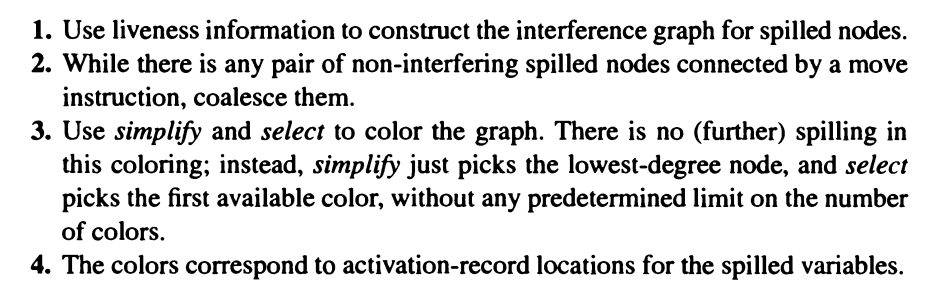
\includegraphics[width=.9\linewidth]{Register Allocation (11)/screenshot_2018-11-19_11-13-28.png}
\end{center}
\begin{itemize}
\item Should done before generating the spill instructions and regenerating the the register-temporary interference graph
\end{itemize}

\subsection{Precolored nodes}
\label{sec:org4e46906}
\subsubsection{General}
\label{sec:orge360ac5}
\begin{itemize}
\item Some temporaries are precolored since they represent machine registers
\begin{itemize}
\item e.g. function arguments
\item The \emph{select} and \emph{coalesce} operations can give an ordinary temporary the same color as a precolored as long as they don't interfere
\item For a \(K\) register machine, there will be \(K\) precolored nodes that all interfere with each other
\item Those of the precolored nodes that are not used explicitly will not interfere with any ordinary nodes
\item A machine register used explicitly will have a live range that interferes with any other variable that might happen to be live at the same time
\item A precolored node cannot be simplified and they should not be spilled
\end{itemize}
\end{itemize}

\subsubsection{Temporary Copies of Machine Registers}
\label{sec:orgb595930}
\begin{itemize}
\item The coloring algorithm works by calling  \emph{simplify}, \emph{coalesce} and \emph{split} until only the precolored node remain
\begin{itemize}
\item Then the \emph{select} phase can start adding the other nodes (and coloring them)
\item Since precolored nodes do not spill, the front end must be careful to keep their live range short
\item It can be done by generating MOVE instruction to move values to and from precolored nodes
\end{itemize}
\end{itemize}

\subsubsection{Caller-Save and Callee-Save Registers}
\label{sec:org0c52025}
\begin{itemize}
\item A local variable or compiler temporary that is not live across any procedure call should usually be allocated to a caller-save register
\begin{itemize}
\item In this case no saving and restoring of register will be necessary at all
\end{itemize}

\item Any variable that is live across several procedure calls should be kept in a callee-save register
\begin{itemize}
\item Since then only one save/restore will be necessary
\end{itemize}

\item The register allocator should allocate variable to registers using this criterion
\begin{itemize}
\item To do this with a graph-coloring allocator the \texttt{CALL} instructions in the \texttt{Assem} language have been annotated to interfere with all the caller-save registers
\end{itemize}
\end{itemize}

\section{Garbage Collection (13)}
\label{sec:org6b8ebe1}
\subsection{General}
\label{sec:org500e045}
\begin{itemize}
\item Heap-allocated records that are not reachable by any chain of points from program variables are \textbf{Garbage}
\begin{itemize}
\item The memory occupied by garbage should be reclaimed for use in allocating new records
\item This process is called \textbf{Garbage Collection}
\item It is not performed by the compiler but by the runtime system
\item We will require the compile to guarantee that any live record is \textbf{reachable}
\item The number of reachable records that are not live should be minimized
\end{itemize}
\end{itemize}

\subsection{Mark-And-Sweep Collection}
\label{sec:orgce8b9e1}
\subsubsection{General}
\label{sec:org08f5f67}
\begin{center}
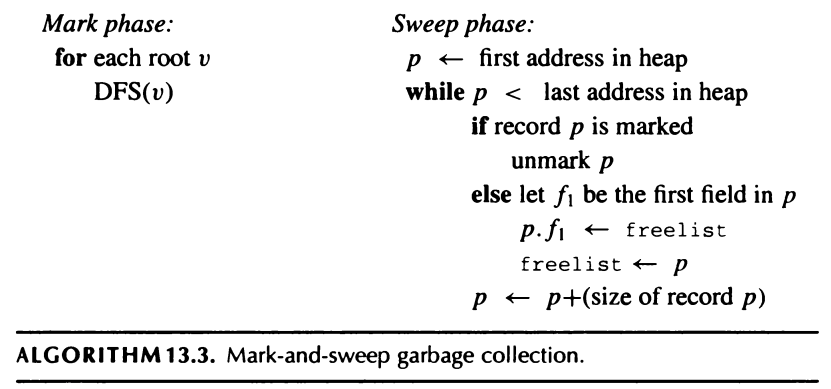
\includegraphics[width=.9\linewidth]{Garbage Collection (13)/screenshot_2018-11-25_10-44-39.png}
\end{center}

\begin{itemize}
\item Program variables and heap-allocated records form a directed graph 
\begin{itemize}
\item The variables are roots of this graph
\item A node \(n\) is reachable if there is a path of directed edges \(r \to \dots \to n\) starting at some root \(r\)
\item A graph-search algorithm such as DFS can mark all reachable nodes
\item Any node not marked must be garbage and should be reclaimed
\begin{itemize}
\item It can be done by a \textbf{sweep} of the entire heap from the first address to the last looking at nodes that are not marked
\item These nodes are garbage and can be linked together in a linked list (the freelist)
\end{itemize}
\item The sweep phase should also unmark all marked nodes in preparation for the next garbage collection
\item After the garbage collection the program resumes execution
\item Whenever the program wants to heap-allocate a new record it gets a record from the freelist
\begin{itemize}
\item When it becomes empty it is a good time to do another garbage collection
\end{itemize}
\item If there are \(R\) words of reachable data in a heap of size \(J\) the cost of a garbage collection is \(O(R+H)\)
\end{itemize}
\end{itemize}

\subsubsection{Using an explicit stack}
\label{sec:orge551efb}
\begin{center}
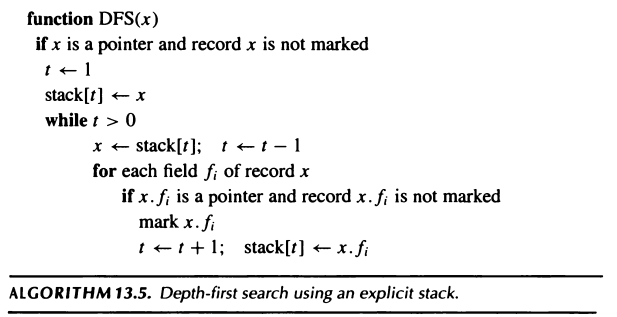
\includegraphics[width=.9\linewidth]{Garbage Collection (13)/screenshot_2018-11-25_10-58-47.png}
\end{center}
\begin{itemize}
\item The DFS algorithm is recursive and the maximum depth of its recursion is as long as the longest path in the graph of reachable data
\item There could be a path of length \(H\) in the worst case
\begin{itemize}
\item Meaning the stack of the activation records would be larger than the entire heap
\end{itemize}
\item To solve this problem an explicit stack is used instead of recursion
\begin{itemize}
\item The stack could still grow to size \(H\)
\item This is \(H\) words and not \(H\) activation records
\end{itemize}
\end{itemize}

\subsubsection{Pointer reversal}
\label{sec:org3c184b4}
\begin{center}
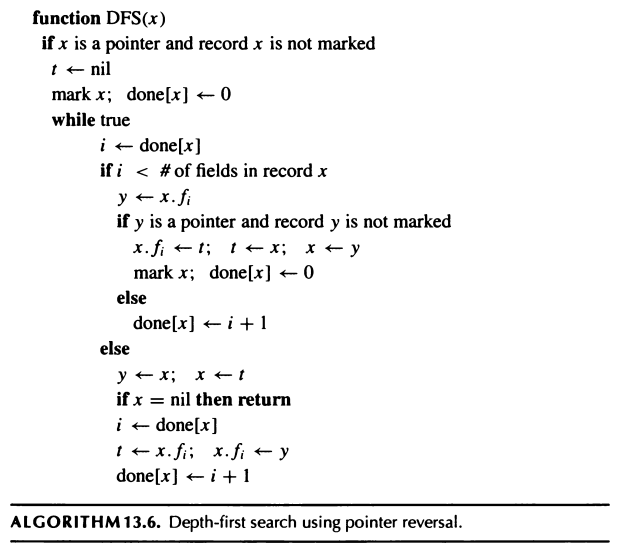
\includegraphics[width=.9\linewidth]{Garbage Collection (13)/screenshot_2018-11-25_11-00-08.png}
\end{center}
\begin{itemize}
\item After the contents of field \(x.f_1\) has been pushed to the stack the algorithm will never look at the original location \(x.f_i\)
\begin{itemize}
\item It means we can use \(x.f_i\) to store one element of the stack itself
\item \(x.f_i\) will be made to point back to the record from which \(x\) was reached
\item When the stack is popped the field \(x.f_i\) will be restored to its original value
\item The algorithm requires a field in each record called \emph{done}
\begin{itemize}
\item It should indicate how many fields in that record have been processed
\item This only takes a few bits per record
\end{itemize}
\item The variable \(t\) servers as the top of the stack
\begin{itemize}
\item Every record \(x\) on the stack is already marked and it \(i=\text{done}[x]\) then \(x.f_i\) is the stack link to the next node down
\item When popping the stack, \(x.f_i\) is restored to its original value
\end{itemize}
\end{itemize}
\end{itemize}

\subsubsection{An array of freelists}
\label{sec:org3abe8a9}
\begin{itemize}
\item The sweep phase is the same no matter which marking algorithm is used
\begin{itemize}
\item It just puts the unmarked records on the freelist, and unmarks the marked records
\end{itemize}
\item If records are of many different sizes, a simple linked list will not be very efficient for the allocator
\begin{itemize}
\item Since when allocating a record of size \(n\), we may have to search a long way down the list for a free block of that size
\end{itemize}
\item A good solution is to have an array of several freelist
\begin{itemize}
\item \(\text{freelist}[i]\) is a linked list of all records of size \(i\)
\end{itemize}
\item The program can allocate a node of size \(i\) just by taking the head of \(\text{freelist}[i]\)
\item The sweep phase of the collector can put each node of size \(j\) at the head of \(\text{freelist}[j]\)
\item If the program attempts to allocate from an empty \(\text{freelist}[i]\),it can try to grab a larger record from \(\text{freelist}[j]\) (for \(j > i\)) and split it
\begin{itemize}
\item Putting the unused potion back on \(\text{freelist}[j-i]\)
\item If this fails it is time to call the garbage collector to replenish the freelists
\end{itemize}
\end{itemize}

\subsubsection{Fragmentation}
\label{sec:org5878f64}
\begin{itemize}
\item I can happen that the program want allocate a record of size \(n\) but there are many smaller that \(n\) 
\begin{itemize}
\item This is called \textbf{external fragmentation}
\begin{itemize}
\item \textbf{Internal fragmentation} occurs when the program uses a too-large record without spliting it
\end{itemize}
\end{itemize}
\end{itemize}

\subsection{Reference Counts}
\label{sec:org615e0e0}
\begin{itemize}
\item Garbage collection can be done directly by keeping track of how many pointers point to each record
\begin{itemize}
\item This is the \textbf{reference count} of the record and it is stored with each record
\item The compiler emits extra instructions so whenever \(p\) is stored into \(x.f_i\)
\begin{itemize}
\item The reference count of \(p\) is incremented
\item The reference count of what \(x.f_i\) previously pointed to decremented
\end{itemize}
\item If the decremented reference count of some record reaches zero then \(r\) is put on the freelist and all other records that \(r\) points to have their reference counts decremented
\item Instead of decrementing the counts of \(r.f_i\) when \(r\) is put on the freelist it is better to do recursive decrementing when \(r\) is removed from the freelist for two reasons
\begin{enumerate}
\item It breaks up the "recursive decrementing" work into shorter pieces
\begin{itemize}
\item This makes the program run more smoothly
\end{itemize}
\item The compiler must emit code (at each decrement) to check whether the count has reached zero and put the record on the freelist
\begin{itemize}
\item The recursive decrementing will only be done in one place the allocator
\end{itemize}
\end{enumerate}
\item There are two major problems with reference counting
\begin{enumerate}
\item Cycles of garbage cannot be reclaimed
\begin{itemize}
\item e.g. a loop of list cells that are not reachable from program variables but each has a reference count of \(1\)
\end{itemize}
\item Incrementing the reference counts is very expensive
\begin{itemize}
\item Since in place of the single machine instruction \(x.f_i \leftarrow p\) the execute
\end{itemize}
\end{enumerate}
\end{itemize}
\end{itemize}
\begin{center}
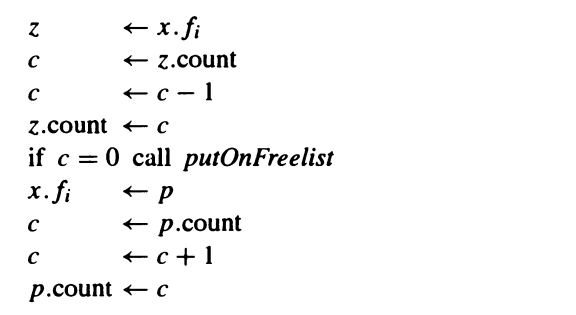
\includegraphics[width=.9\linewidth]{Garbage Collection (13)/screenshot_2018-11-25_11-26-10.png}
\end{center}

\begin{itemize}
\item A naive reference counter will increment and decrement the counts on every since assignment to a program variable
\begin{itemize}
\item Since this would be very expensive many increments and decrements are eliminated using dataflow analysis
\begin{itemize}
\item As a pointer value is fetched and then propagated through local variables, the compile can aggregate the many change in the count to a since increment
\end{itemize}
\item Even with this technique there are many ref-counts increments and decrements that remain and their cost is very high
\item There are two possible possible solutions to the cycles problem
\begin{enumerate}
\item Simply require the programmer to explicitly break all cycles when she is done with the data structure
\begin{itemize}
\item It is less annoying than putting explicit free calls
\item It is hardly elegant
\end{itemize}
\item Coming reference counting with an occasional mark-sweep collection
\end{enumerate}
\item As a whole the problems with reference counting outweigh its advantages
\begin{itemize}
\item It is rarely used
\end{itemize}
\end{itemize}
\end{itemize}

\subsection{Copying Collection}
\label{sec:org5ba001d}
\subsubsection{General}
\label{sec:org70c7df8}
\begin{center}
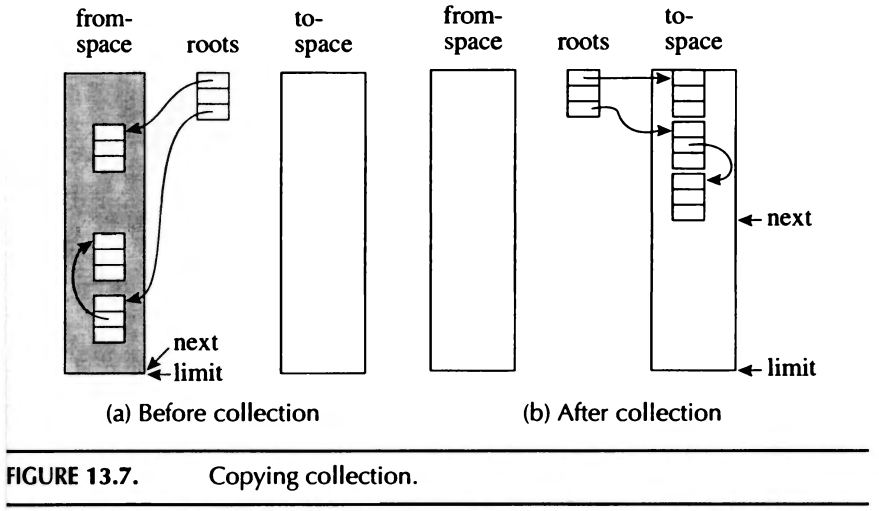
\includegraphics[width=.9\linewidth]{Garbage Collection (13)/screenshot_2018-11-25_16-20-05.png}
\end{center}
\begin{itemize}
\item The reachable part of the heap is a directed graph with records as nodes and pointers as edges and program variables as roots
\item \textbf{Copying garbage collection} traverses this graph in a part of the heap (called \textbf{from-space)} building a isomorphic copy in a fresh area of the head (called \textbf{to-space})
\begin{itemize}
\item The to-space copy is \textbf{compact}, occupying contiguous memory without fragmentation
\item The roots are made to point at the to-space copy
\item Then the entire from-space is unreachable
\begin{itemize}
\item Garbage plus the previously reachable graph
\end{itemize}
\item It does not have a fragmentation problem
\item Eventually the program will allocate enough that \texttt{next} reaches \texttt{limit}
\begin{itemize}
\item The another garbage collection is needed
\item The roles of to and from space are swapped
\end{itemize}
\end{itemize}

\item \textbf{Initiating a collection:} to start a new collection, the pointer \texttt{next} is initialized to point at the beginning of to-space
\begin{itemize}
\item As a reachable record is found in the from space it is copied to to-space at position \texttt{next}, and \texttt{next} incremented by the size of the record
\end{itemize}
\end{itemize}

\subsubsection{Forwarding}
\label{sec:org0e68759}
\begin{center}
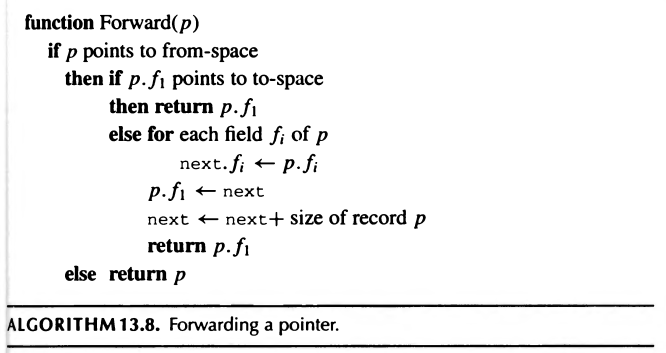
\includegraphics[width=.9\linewidth]{Garbage Collection (13)/screenshot_2018-11-25_16-36-53.png}
\end{center}
\begin{itemize}
\item The basic operation of copying collection is forwarding a pointer
\begin{itemize}
\item That is, given a pointer \(p\) that points to from-space, make \(p\) point to to-space
\item There are three cases:
\begin{enumerate}
\item If \(p\) points to a from-space record that has already been copied
\begin{itemize}
\item Then \(p.f_1\) is a special \emph{forwarding pointer} that indicates where the copy is
\item The forwarding pointer can be identified just by the fact that it points within the to-space, as no ordinary from-space field could point there
\end{itemize}
\item If \(p\) points to a from-space record that has not yet been copied
\begin{itemize}
\item It is copied to location \texttt{next}
\item The forwarding pointer is installed into \(p.f_1\)
\item It is all right to overwrite the \(f_1\) field of the old record because all the data have already been copied to the to-space of \texttt{next}
\end{itemize}
\item If \(p\) is not a pointer at all, or if it points outside from space, then forwarding \(p\) does nothing
\end{enumerate}
\end{itemize}
\end{itemize}

\subsubsection{Cheney's algorithm}
\label{sec:org869e25c}
\begin{center}
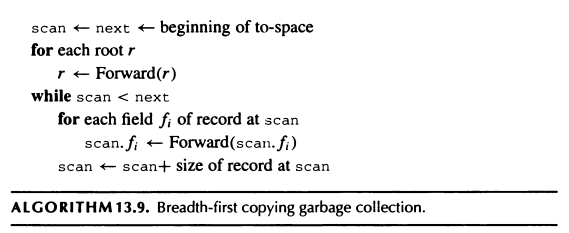
\includegraphics[width=.9\linewidth]{Garbage Collection (13)/screenshot_2018-11-25_16-41-02.png}
\end{center}

\begin{itemize}
\item The simplest algorithm for copying collection uses BFS to traverse the reachable data 
\begin{itemize}
\item The roots are forwarded
\begin{itemize}
\item This copies a few records to to-space thereby incrementing \texttt{next}
\end{itemize}
\item The area between \texttt{scan} and \texttt{next} contains records that have been copied to to-space
\begin{itemize}
\item The fields has not yet been forwarded
\item These fields point in general to from-space
\end{itemize}
\item The area between the beginning of to-space and \texttt{scan} contains records that have been copied and forwarded
\begin{itemize}
\item All pointers in this area point to to-space
\end{itemize}
\item The while loop of algorithm moves \texttt{scan} toward next
\begin{itemize}
\item Copying records will cause next to move also
\item Eventually \texttt{scan} catches up with next after all reachable data are copied to to-space
\end{itemize}
\item It requires no external stack and no pointer reversal
\begin{itemize}
\item It uses the to-space area between \texttt{scan} and \texttt{next} as the queue of its BFS
\item It makes it simpler to implement than DFS with pointer reversal
\end{itemize}
\end{itemize}
\end{itemize}

\subsubsection{Locality of reference}
\label{sec:org6545893}
\begin{itemize}
\item Pointer data structures copied by BFS have poor locality of reference
\begin{itemize}
\item Since the records near each other are those whose distance from the roots are equal
\item Record near each other are not likely to be related
\end{itemize}

\item In a computer system with virtual memory or memory a memory cache good locality of reference is important
\begin{itemize}
\item After the program fetches address \(a\) then the memory subsystem expects addresses near \(a\) to be fetched soon
\item This ensures that the entire page or cache line containing nearby addresses can be quickly accessed
\end{itemize}
\end{itemize}

\begin{center}
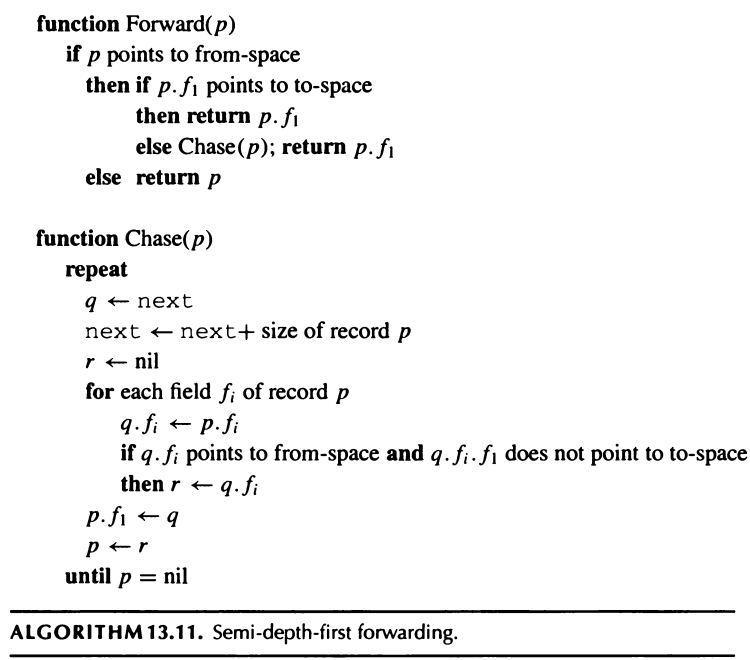
\includegraphics[width=.9\linewidth]{Garbage Collection (13)/screenshot_2018-11-25_17-07-23.png}
\end{center}
\begin{itemize}
\item Depth-first copying given better locality, since each object \(a\) tend to be adjacent to its first child \(b\)
\begin{itemize}
\item This is unless \(b\) is adjacent to another "parent" \(a'\)
\item A hybrid partly depth first and partly breadth first algorithm can provide acceptable locality
\begin{itemize}
\item The basic idea is to use breadth-first copying but whenever an object is copied see if some child can be copied near it
\end{itemize}
\end{itemize}
\end{itemize}

\subsection{Generational Collection}
\label{sec:org2b41a7a}
\begin{itemize}
\item Since in many programs new objects are likely to die soon whereas an objects still reachable after many collections will probably survive for many more collections 
\begin{itemize}
\item The collector should concentrate its effort on "young data"
\item Since there is a higher proportion of garbage
\item A heap is divided into \textbf{generations}
\begin{itemize}
\item The youngest objects in generation \(G_0\)
\item Ever object in generation \(G_1\) is older than any object in \(G_0\)
\item Everything in \(G_2\) is older than \(G_1\) and so on
\end{itemize}
\item To collect just \(G_0\) just start from the roots and either depth-first marking or breadth-first copying
\begin{itemize}
\item The roots are not just program variables the include any pointer within \(G_1,G_2, \dots\)
\item If there are too many of these then processing the roots will take longer than traversal of reachable objects within \(G_0\)
\item Its rare for an older object to point to a much younger object
\item To void searching all of \(G_1, G_2, \dots\) for root of \(G_0\) we make the compiled program remember where there are pointers from old objects to new once
\end{itemize}
\item There are several ways of remembering
\begin{itemize}
\item \textbf{Remembered list:} The compiler generates code, after each \emph{update} store of the form \(b.f_i \leftarrow a\) to put \(b\) into a vector of updated object
\begin{itemize}
\item At each garbage collection the collector scans the remembered list loking for old objects \(b\) that point into \(G_0\)
\end{itemize}
\item \textbf{Remembered set}: Like the remembered list, but uses a bit within object \(b\) to remember to record that \(b\) is already in the vector
\begin{itemize}
\item The code generated by the compiler can check this bit to avoid duplicate reference to \(b\) in the vector
\end{itemize}
\item \textbf{Card marking:} Divide the memory into logical "cards" of size \(2^k\) bytes
\begin{itemize}
\item An object can occupy part of a card or start in the middle of one card and continue onto the next
\item Whenever address \(b\) is updated the card containing that address is marked
\item There is an array of bytes that server as marks
\item The byte index can be found by shifting address \(b\) right by \(k\) bits
\end{itemize}
\item \textbf{Page marking:} Is like card marking, but if \(2^k\) is the page size the computers virtual memory system can be used instead of extra instructions generated by the compiler
\begin{itemize}
\item Updating an old generation sets a dirty bit for that page
\end{itemize}
\end{itemize}
\item When a garbage collection begins the remembered set tells which objects of the old generation can possible contains pointer into \(G_0\) are scanned for roots
\begin{itemize}
\item When using the copying collection only \(G_0\) are copied
\item The marking algorithm does not mark old generation records
\item After several collections of \(G_0\), generation \(G_1\) may have accumulated a lot of garbage
\begin{itemize}
\item Since \(G_0\) may contain many pointers into \(G_1\) it is best to collect \(G_0\) and \(G_1\)
\item The remembered set must be scanned for roots contained in \(G_2, G_3, \dots\)
\end{itemize}
\item Each older generation should be exponentially bigger than the previous one
\item An object should be promoted from \(G_i\) to \(G_{i+1}\) when it survives two or three collections of \(G_i\)
\item If the program does many more updates than fresh allocations generational collection may be more expensive than non generation collection
\end{itemize}
\end{itemize}
\end{itemize}

\subsection{Incremental Collection}
\label{sec:org4b772cc}
\begin{itemize}
\item Even if the overall garbage collection time is only a few percent of the computation time, the collector will occasionally interrupt the program for long periods
\begin{itemize}
\item For interactive or real-time programs this is undirable
\item Incremental or concurrent algorithm s interleave garbage collection work with program execution to avoid long interruptions
\end{itemize}
\end{itemize}

\begin{center}
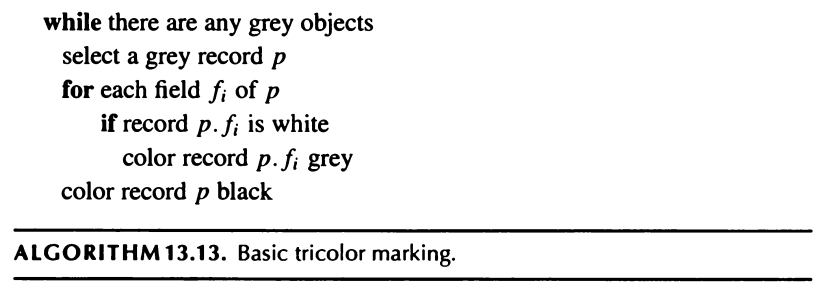
\includegraphics[width=.9\linewidth]{Garbage Collection (13)/screenshot_2018-11-26_10-48-43.png}
\end{center}

\begin{itemize}
\item Terminology
\begin{itemize}
\item The \textbf{collector} tries to collect garbage
\item The compiled program keeps changing the graph of reachable data so it is the \textbf{mutator}
\item An \textbf{incremental} algorithm is one in which the collector operates only when the mutator requests it
\item A \textbf{concurrent} algorithm is one where the collector can operate between or during any instructions executed by the mutator
\end{itemize}

\item \textbf{Tricolor marking.} In a mark-sweep or copying garbage collection, there are three classes of records:
\begin{itemize}
\item \textbf{White} objects are not yet visited by the depth-first or breadth-first search
\item \textbf{Grey} objects have been visited (marked or copied), but their children have not yet been examined
\begin{itemize}
\item In mark-sweep collection, these objects are on the stack
\item In Cheney's copying collection they are between \texttt{scan} and \texttt{next}
\end{itemize}
\item \textbf{Black} objects have been marked an their children also marked
\begin{itemize}
\item In mark-sweep collection, they have already been popped of the stack
\item In Cheney's copying collection they have already been scanned
\end{itemize}
\end{itemize}

\item The collection starts with all objects white
\begin{itemize}
\item The collector executes the basic tricolor marking algorithm
\item Blackening gray objects and graying their white children
\item In changing an object from gray to black is removing it from the stack or queue
\item When there are no gray objects then all the white objects must be garbage
\end{itemize}

\item All the algorithms preserve two natural invariants
\begin{enumerate}
\item No black object points to a white object
\item Every gray object is on the collector's data structure
\begin{itemize}
\item Called the gray set
\end{itemize}
\end{enumerate}

\item While the collector operates the mutator creates new object and updates pointer fields of existing objects
\begin{itemize}
\item If the mutator breaks one of the invariants the collection algorithm will not work
\item Most incremental and concurrent collection algorithm are based on techniques which allows the mutator to get work done while preserving invariants
\end{itemize}

\item Examples of incremental and concurrent collection algorithms:
\end{itemize}
\begin{center}
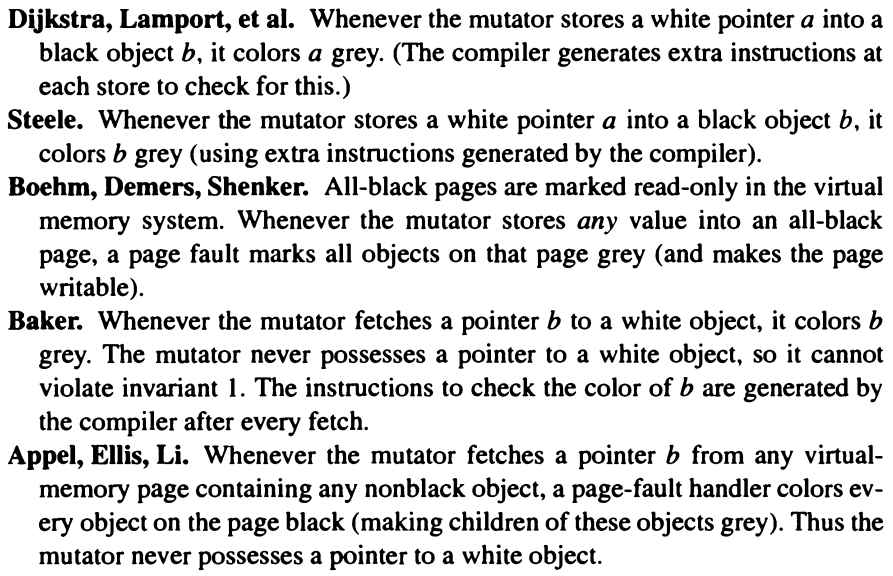
\includegraphics[width=.9\linewidth]{Garbage Collection (13)/screenshot_2018-11-26_11-08-23.png}
\end{center}
\begin{itemize}
\item The first three are \textbf{writer-barrier} algorithms
\begin{itemize}
\item It means that each store by the mutator must be checked to make sure that an invariant is preserved
\end{itemize}

\item The last two are \textbf{read-barrier} algorithms
\begin{itemize}
\item It means that fetch instruction are the one that must be checked
\end{itemize}

\item Any implementation of a write or read barrier must synchronize with the collector
\begin{itemize}
\item Software implementations of the read or write barrier will need to use explicit synchronization which can be expensie
\item Implementations using virtual-memory hardware can take advantage of the synchronization implicit in a page fault
\begin{itemize}
\item i.e. if the mutator faults on a page the operating system will ensure that no other process has access to that page before processing the fault
\end{itemize}
\end{itemize}
\end{itemize}

\subsection{Backer's Algorithm}
\label{sec:org6716edf}
\begin{itemize}
\item \textbf{Backer's Algorithm} illustrates the details of instrumental collection
\begin{itemize}
\item It is based on Cheney's copying algorithm
\item It forward reachable object from-space to to-space
\item It is compatible with generational collection
\begin{itemize}
\item From-space and to-space might be for generation \(G_0\), or might be \(G_0 + \cdots + G_k\)
\end{itemize}
\item To initiate a garbage the roles of the from-space and to-space are swapped and all the roots are forwarded this is called the flip 
\begin{itemize}
\item The mutator is then resumed
\item Each time the mutator calls the allocator to get a new record, a few pointers at \texttt{scan} are scanned, so that \texttt{scan} advances toward next
\begin{itemize}
\item The new record is allocated at the end of the to-space by decrementing \texttt{limit} by the appropriate amount
\end{itemize}
\item The invariant is that the mutator has pointers only to to-space
\begin{itemize}
\item Thus when the mutator allocates and initializes a new record that record need not to be scanned
\end{itemize}
\item When the mutator stores a pointer into an old record it is only storing the to-space pointer
\item If hte mutator fetches a field of a record it might invariant
\begin{itemize}
\item Each fetch is followed by two or three instruction that check wether the fetched pointer points to from-space
\item If so, the pointer must be forwarded immediately using the standard forward algorithm
\end{itemize}
\item For every word allocated, the allocated must advance \texttt{scan} by at least one word
\begin{itemize}
\item When \texttt{scan=next} the collection terminates until the allocator runs out of space
\end{itemize}
\item The largest cost of the Baker's algorithm is the extra instructions after every fetch
\end{itemize}
\end{itemize}
\end{itemize}

\subsection{Interface to the Compiler}
\label{sec:org0816ebb}
\subsubsection{General}
\label{sec:org0e16c43}
\begin{itemize}
\item The compiler for a garbage-collected language interacts with the garbage collector by generating code that allocates record
\begin{itemize}
\item By describing locations of roots for each garbage-collection cycle
\item By describing the layout of data records on the heap
\item For some versions of incremental collection the compiler must also generate instructions to implement a read barrier or write barrier
\end{itemize}
\end{itemize}

\subsubsection{Fast Allocation}
\label{sec:org13f4d37}
\begin{itemize}
\item Some programming languages and some programs allocate heap data very rapidly
\begin{itemize}
\item To minimize the cost of the garbage collector \textbf{copying collection} should be used so that the allocation space is a contiguous free region
\item The next free location is \texttt{next}
\item The end of the region is \texttt{limit}
\item To allocate one record of size \(N\) the steps are
\end{itemize}
\end{itemize}
\begin{center}
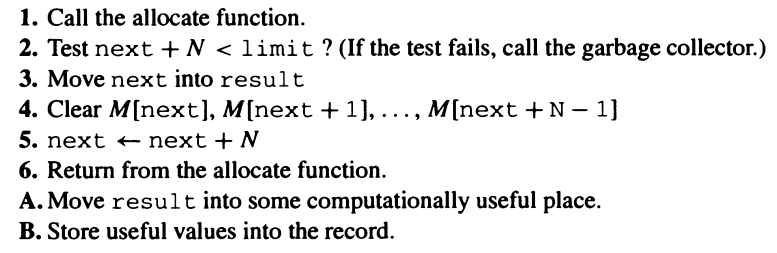
\includegraphics[width=.9\linewidth]{Garbage Collection (13)/screenshot_2018-11-26_12-21-22.png}
\end{center}
\begin{itemize}
\item Steps 1 and 6 should be eliminated by inline expanding the allocate function at each place where a record is allocated
\item Step 3 can often by eliminated by combining it with step A
\item Step 4 can be eliminated in facor of step B
\item Steps 2 and 5 cannot be eliminated but if there is more than once allocation in the same basic block then the comparison and increment can be shared among multiple allocations
\item By keeping \texttt{next} and \texttt{limit} in registers steps 2 and 5 can be done in a total of three instructions
\item By using these techniques the cost of garbage collection can be reduced to 4 instructions
\end{itemize}

\subsubsection{Describing Data Layout}
\label{sec:orga5b7271}
\begin{itemize}
\item The collector must be able to operate on records of all types: \texttt{list}, \texttt{tree} or whatever the program has declared
\begin{itemize}
\item It must be able to determine the number of fields in each record and whether each field is a pointer
\item In statically typed languages or object oriented the simplest way to identify heap objects is to have the first word of every object point to a special type or class descriptor record
\begin{itemize}
\item For statically typed language is an overhead of one word
\item For object oriented languages this descriptor pointer needs to be in every object just to implement dynamic method lookup
\begin{itemize}
\item No additional per-object overhead attributable to garbage collection
\end{itemize}
\end{itemize}
\item The type- or class-descriptor must be generated by the compiler from the semantic analysis phase of the compiler
\begin{itemize}
\item The descriptor-pointer will be the argument to the runtime systems \texttt{alloc} function
\end{itemize}
\item The compiler must identify to the collector every pointer containing temporary and local variable
\begin{itemize}
\item This is whether it is in a register or in an activation record
\begin{itemize}
\item Since the set of live temporaries can change at every instruction
\item The pointer map is different at every point in the program
\item It is simpler to describe the pointer map only at points where the garbage collector can begin
\begin{itemize}
\item Calls to the \texttt{alloc} function
\end{itemize}
\end{itemize}
\item Any function might be calling a function that in turn calls \texttt{alloca}
\item The pointer map must described at each function call
\end{itemize}
\item It is best keyed by return address
\begin{itemize}
\item A function call at location \(a\) is best described by its return address directly after \(a\)
\end{itemize}
\item The data structure maps  return addresses to live-pointer sets
\begin{itemize}
\item For each pointer that is live immediately after the call the pointer map tells its location
\end{itemize}
\item To find all the roots the collector starts at the top of the stack and scans downward frame by frame
\item Callee-save registers need special handling
\begin{itemize}
\item They must be inherited from the calling function
\end{itemize}
\end{itemize}
\end{itemize}

\subsubsection{Derived Pointers}
\label{sec:org0ba3f56}
\begin{itemize}
\item \(t_1\) is derived from the base pointer \(a\) if it points to a place in that record
\begin{itemize}
\item The pointer map must identify each derived pointer and tell the base pointer from which it is derived
\item When the collector relocates \(a\) to address \(a'\) it just adjeust \(t_1\) to point to address \(t_1+a^{'}-a\)
\end{itemize}
\end{itemize}

\section{Exam}
\label{sec:org18d72b2}
\begin{itemize}
\item Læs om recursive descent parsing
\end{itemize}
\end{document}
%%% Local Variables:
%%% mode: latex
%%% TeX-master: t
%%% End:
